\documentclass[a4paper,twoside,12pt]{article}
\usepackage[hmargin={12mm,55mm},vmargin=10mm,footskip=7mm,asymmetric]{geometry}
\usepackage{amsmath}
\usepackage{amssymb}
\usepackage{tikz}
\usepackage{xcolor}
\usepackage{comment}
\usepackage{adjustbox}
\usepackage{iftex}
\ifPDFTeX
\usepackage[T1]{fontenc}
\usepackage[utf8]{inputenc}
\else
\usepackage[no-math]{fontspec}
\fi
\usepackage{libertine}

\makeatletter
\let\_\relax
\DeclareRobustCommand{\_}{%
  \leavevmode\vbox{%
    \hrule\@width.4em
          \@height-.16ex
          \@depth\dimexpr.16ex+.28pt\relax}}
\makeatother

\newcommand\Tstrut{\rule{0pt}{2.4ex}}
\newcommand\Bstrut{\rule[-1.1ex]{0pt}{0pt}}

\tikzset{
   tableaulabel/.style={draw=black!30, fill=gray!4, inner sep = 0.5mm, outer sep = 3mm, circle},
   tableau/.style={draw=black!30, fill=gray!4, inner sep = 3mm, outer sep = 3mm, rounded corners=3mm, align=center},
}

\definecolor{greycolour}{rgb}{0.6, 0.6, 0.6}
\newcommand\grey[1]{{\color{greycolour}{#1}}}

\setlength\marginparwidth{45mm}

\newenvironment{fit}{\begin{adjustbox}{max width=\textwidth,max totalheight=\textheight,keepaspectratio}}{\end{adjustbox}}


\ifdefined\showsteps
  \includecomment{steps}
\else
  \excludecomment{steps}
\fi

\raggedbottom

\begin{document}

{\begin{center} \large \textbf{If $f$ is a surjection then $f(A)\cap f(B)\subset f(A\cap B)$}\end{center}}\nopagebreak[4]

\begin{center}
\begin{minipage}{120mm}
Let $x$ be an element of $f(A)\cap f(B)$. Then $x\in f(A)$ and $x\in f(B)$. That is, there exists $y\in A$ such that $f(y) = x$ and there exists $z\in B$ such that $f(z) = x$. We would like to find $u\in A\cap B$ s.t. $f(u) = x$. But $u\in A\cap B$ if and only if $u\in A$ and $u\in B$.
\end{minipage}
\end{center}

\bigskip
\begin{steps}
\begin{fit}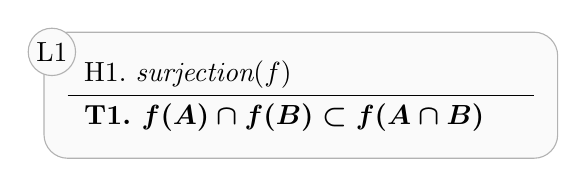
\begin{tikzpicture}[baseline=(main.base)]%
\node[tableau] (main) {%
\\

\begin{tabular}{ll}%
H1.\ $\textit{surjection}(f)$&
\Bstrut\\\hline\Tstrut
\textbf{\boldmath T1.\ $\textrm{$f(A)\cap f(B)\subset f(A\cap B)$}$\unboldmath }&\textbf{\boldmath \unboldmath }
\end{tabular}%
};%
\node[tableaulabel] at (main.north west) [xshift=4mm, yshift=-5.5mm] {L1};
\end{tikzpicture}%
\end{fit}
\smallskip

\noindent1. Expand pre-universal target T1.\nopagebreak[4] 
\marginpar{}\nopagebreak[4] 
\smallskip\nopagebreak[4] 

\begin{fit}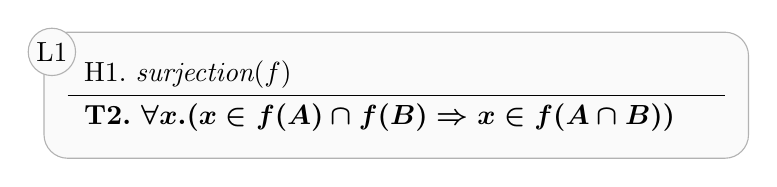
\begin{tikzpicture}[baseline=(main.base)]%
\node[tableau] (main) {%
\\

\begin{tabular}{ll}%
H1.\ $\textit{surjection}(f)$&
\Bstrut\\\hline\Tstrut
\textbf{\boldmath T2.\ $\forall x.(\textrm{$x\in f(A)\cap f(B)$}\Rightarrow \textrm{$x\in f(A\cap B)$})$\unboldmath }&\textbf{\boldmath \unboldmath }
\end{tabular}%
};%
\node[tableaulabel] at (main.north west) [xshift=4mm, yshift=-5.5mm] {L1};
\end{tikzpicture}%
\end{fit}
\smallskip

\noindent2. Apply `let' trick and move premise of universal-conditional target T2 above the line.\nopagebreak[4] 
\marginpar{Let $x$ be an element of $f(A)\cap f(B)$.}\nopagebreak[4] 
\smallskip\nopagebreak[4] 

\begin{fit}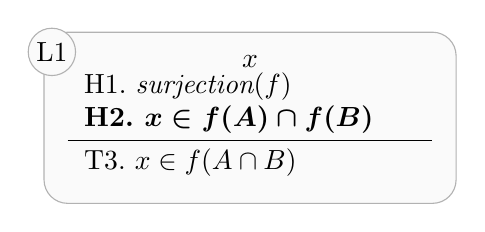
\begin{tikzpicture}[baseline=(main.base)]%
\node[tableau] (main) {%
$x$\\

\begin{tabular}{ll}%
H1.\ $\textit{surjection}(f)$&\\
\textbf{\boldmath H2.\ $\textrm{$x\in f(A)\cap f(B)$}$\unboldmath }&\textbf{\boldmath \unboldmath }
\Bstrut\\\hline\Tstrut
T3.\ $\textrm{$x\in f(A\cap B)$}$&
\end{tabular}%
};%
\node[tableaulabel] at (main.north west) [xshift=4mm, yshift=-5.5mm] {L1};
\end{tikzpicture}%
\end{fit}
\smallskip

\noindent3. Quantifier-free expansion of hypothesis H2.\nopagebreak[4] 
\marginpar{Since $x\in f(A)\cap f(B)$, $x\in f(A)$ and $x\in f(B)$.}\nopagebreak[4] 
\smallskip\nopagebreak[4] 

\begin{fit}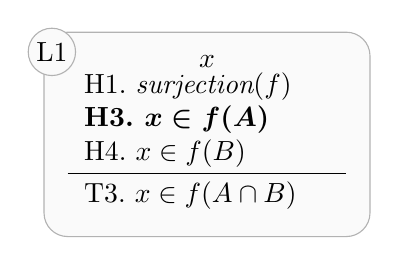
\begin{tikzpicture}[baseline=(main.base)]%
\node[tableau] (main) {%
$x$\\

\begin{tabular}{ll}%
H1.\ $\textit{surjection}(f)$&\\
\textbf{\boldmath H3.\ $\textrm{$x\in f(A)$}$\unboldmath }&\textbf{\boldmath \unboldmath }\\
H4.\ $\textrm{$x\in f(B)$}$&
\Bstrut\\\hline\Tstrut
T3.\ $\textrm{$x\in f(A\cap B)$}$&
\end{tabular}%
};%
\node[tableaulabel] at (main.north west) [xshift=4mm, yshift=-5.5mm] {L1};
\end{tikzpicture}%
\end{fit}
\smallskip

\noindent4. Expand pre-existential hypothesis H3.\nopagebreak[4] 
\marginpar{By definition, since $x\in f(A)$, there exists $y\in A$ such that $f(y) = x$.}\nopagebreak[4] 
\smallskip\nopagebreak[4] 

\begin{fit}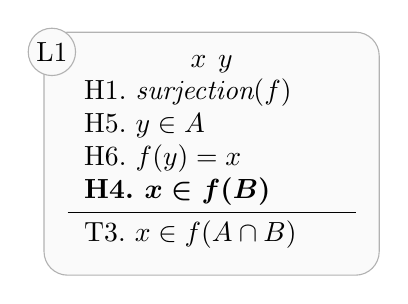
\begin{tikzpicture}[baseline=(main.base)]%
\node[tableau] (main) {%
$x$\hspace{1.5mm}$y$\\

\begin{tabular}{ll}%
H1.\ $\textit{surjection}(f)$&\\
H5.\ $\textrm{$y\in A$}$&\\
H6.\ $\textrm{$f(y) = x$}$&\\
\textbf{\boldmath H4.\ $\textrm{$x\in f(B)$}$\unboldmath }&\textbf{\boldmath \unboldmath }
\Bstrut\\\hline\Tstrut
T3.\ $\textrm{$x\in f(A\cap B)$}$&
\end{tabular}%
};%
\node[tableaulabel] at (main.north west) [xshift=4mm, yshift=-5.5mm] {L1};
\end{tikzpicture}%
\end{fit}
\smallskip

\noindent5. Expand pre-existential hypothesis H4.\nopagebreak[4] 
\marginpar{By definition, since $x\in f(B)$, there exists $z\in B$ such that $f(z) = x$.}\nopagebreak[4] 
\smallskip\nopagebreak[4] 

\begin{fit}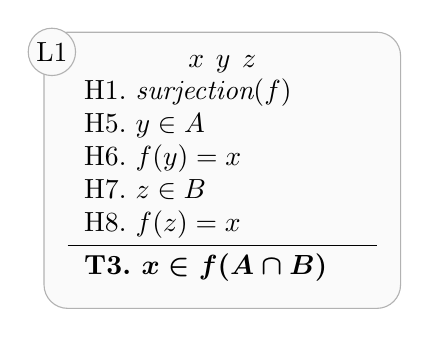
\begin{tikzpicture}[baseline=(main.base)]%
\node[tableau] (main) {%
$x$\hspace{1.5mm}$y$\hspace{1.5mm}$z$\\

\begin{tabular}{ll}%
H1.\ $\textit{surjection}(f)$&\\
H5.\ $\textrm{$y\in A$}$&\\
H6.\ $\textrm{$f(y) = x$}$&\\
H7.\ $\textrm{$z\in B$}$&\\
H8.\ $\textrm{$f(z) = x$}$&
\Bstrut\\\hline\Tstrut
\textbf{\boldmath T3.\ $\textrm{$x\in f(A\cap B)$}$\unboldmath }&\textbf{\boldmath \unboldmath }
\end{tabular}%
};%
\node[tableaulabel] at (main.north west) [xshift=4mm, yshift=-5.5mm] {L1};
\end{tikzpicture}%
\end{fit}
\smallskip

\noindent6. Expand pre-existential target T3.\nopagebreak[4] 
\marginpar{We would like to find $u\in A\cap B$ s.t. $f(u) = x$.}\nopagebreak[4] 
\smallskip\nopagebreak[4] 

\begin{fit}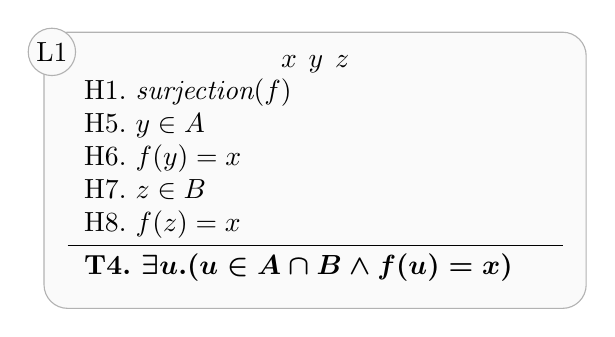
\begin{tikzpicture}[baseline=(main.base)]%
\node[tableau] (main) {%
$x$\hspace{1.5mm}$y$\hspace{1.5mm}$z$\\

\begin{tabular}{ll}%
H1.\ $\textit{surjection}(f)$&\\
H5.\ $\textrm{$y\in A$}$&\\
H6.\ $\textrm{$f(y) = x$}$&\\
H7.\ $\textrm{$z\in B$}$&\\
H8.\ $\textrm{$f(z) = x$}$&
\Bstrut\\\hline\Tstrut
\textbf{\boldmath T4.\ $\exists u.(\textrm{$u\in A\cap B$}\wedge \textrm{$f(u) = x$})$\unboldmath }&\textbf{\boldmath \unboldmath }
\end{tabular}%
};%
\node[tableaulabel] at (main.north west) [xshift=4mm, yshift=-5.5mm] {L1};
\end{tikzpicture}%
\end{fit}
\smallskip

\noindent7. Unlock existential target T4.\nopagebreak[4] 
\marginpar{We would like to find $u\in A\cap B$ s.t. $f(u) = x$.}\nopagebreak[4] 
\smallskip\nopagebreak[4] 

\begin{fit}\begin{tikzpicture}[baseline=(main.base)]%
\node[tableau] (main) {%
$x$\hspace{1.5mm}$y$\hspace{1.5mm}$z$\\

\begin{tabular}{ll}%
H1.\ $\textit{surjection}(f)$&\\
H5.\ $\textrm{$y\in A$}$&\\
H6.\ $\textrm{$f(y) = x$}$&\\
H7.\ $\textrm{$z\in B$}$&\\
H8.\ $\textrm{$f(z) = x$}$&
\Bstrut\\\hline\Tstrut
\begin{tikzpicture}[baseline=(main.base)]%
\node[tableau] (main) {%
$u^\blacklozenge $\\

\begin{tabular}{ll}%

\Bstrut\\\hline\Tstrut
\textbf{\boldmath T5.\ $\textrm{$u^\blacklozenge \in A\cap B$}$\unboldmath }&\textbf{\boldmath \unboldmath }\\
T6.\ $\textrm{$f(u^\blacklozenge ) = x$}$&
\end{tabular}%
};%
\node[tableaulabel] at (main.north west) [xshift=4mm, yshift=-5.5mm] {L2$^\blacklozenge$};
\end{tikzpicture}%

\end{tabular}%
};%
\node[tableaulabel] at (main.north west) [xshift=4mm, yshift=-5.5mm] {L1};
\end{tikzpicture}%
\end{fit}
\smallskip

\noindent8. Quantifier-free expansion of target T5.\nopagebreak[4] 
\marginpar{But $u\in A\cap B$ if and only if $u\in A$ and $u\in B$.}\nopagebreak[4] 
\smallskip\nopagebreak[4] 

\begin{fit}\begin{tikzpicture}[baseline=(main.base)]%
\node[tableau] (main) {%
$x$\hspace{1.5mm}$y$\hspace{1.5mm}$z$\\

\begin{tabular}{ll}%
H1.\ $\textit{surjection}(f)$&\\
H5.\ $\textrm{$y\in A$}$&\\
H6.\ $\textrm{$f(y) = x$}$&\\
H7.\ $\textrm{$z\in B$}$&\\
H8.\ $\textrm{$f(z) = x$}$&
\Bstrut\\\hline\Tstrut
\begin{tikzpicture}[baseline=(main.base)]%
\node[tableau] (main) {%
$u^\blacklozenge $\\

\begin{tabular}{ll}%

\Bstrut\\\hline\Tstrut
T7.\ $\textrm{$u^\blacklozenge \in A$}$&\\
T8.\ $\textrm{$u^\blacklozenge \in B$}$&\\
T6.\ $\textrm{$f(u^\blacklozenge ) = x$}$&
\end{tabular}%
};%
\node[tableaulabel] at (main.north west) [xshift=4mm, yshift=-5.5mm] {L2$^\blacklozenge$};
\end{tikzpicture}%

\end{tabular}%
};%
\node[tableaulabel] at (main.north west) [xshift=4mm, yshift=-5.5mm] {L1};
\end{tikzpicture}%
\end{fit}

No moves possible.
\cleardoublepage

\end{steps}
{\begin{center} \large \textbf{If $f$ is an injection then $f(A)\cap f(B)\subset f(A\cap B)$}\end{center}}\nopagebreak[4]

\begin{center}
\begin{minipage}{120mm}
Let $x$ be an element of $f(A)\cap f(B)$. Then $x\in f(A)$ and $x\in f(B)$. That is, there exists $y\in A$ such that $f(y) = x$ and there exists $z\in B$ such that $f(z) = x$. Since $f$ is an injection, $f(y) = x$ and $f(z) = x$, we have that $y = z$. We would like to find $u\in A\cap B$ s.t. $f(u) = x$. But $u\in A\cap B$ if and only if $u\in A$ and $u\in B$. Since $y = z$, we have that $y\in B$. Therefore, setting $u = y$, we are done.
\end{minipage}
\end{center}

\bigskip
\begin{steps}
\begin{fit}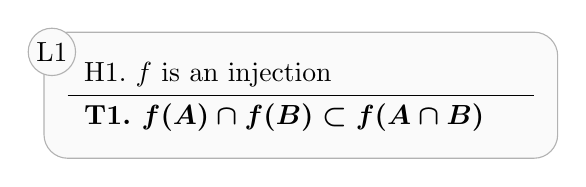
\begin{tikzpicture}[baseline=(main.base)]%
\node[tableau] (main) {%
\\

\begin{tabular}{ll}%
H1.\ $\textrm{$f$ is an injection}$&
\Bstrut\\\hline\Tstrut
\textbf{\boldmath T1.\ $\textrm{$f(A)\cap f(B)\subset f(A\cap B)$}$\unboldmath }&\textbf{\boldmath \unboldmath }
\end{tabular}%
};%
\node[tableaulabel] at (main.north west) [xshift=4mm, yshift=-5.5mm] {L1};
\end{tikzpicture}%
\end{fit}
\smallskip

\noindent1. Expand pre-universal target T1.\nopagebreak[4] 
\marginpar{}\nopagebreak[4] 
\smallskip\nopagebreak[4] 

\begin{fit}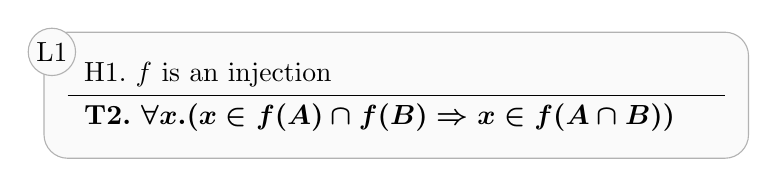
\begin{tikzpicture}[baseline=(main.base)]%
\node[tableau] (main) {%
\\

\begin{tabular}{ll}%
H1.\ $\textrm{$f$ is an injection}$&
\Bstrut\\\hline\Tstrut
\textbf{\boldmath T2.\ $\forall x.(\textrm{$x\in f(A)\cap f(B)$}\Rightarrow \textrm{$x\in f(A\cap B)$})$\unboldmath }&\textbf{\boldmath \unboldmath }
\end{tabular}%
};%
\node[tableaulabel] at (main.north west) [xshift=4mm, yshift=-5.5mm] {L1};
\end{tikzpicture}%
\end{fit}
\smallskip

\noindent2. Apply `let' trick and move premise of universal-conditional target T2 above the line.\nopagebreak[4] 
\marginpar{Let $x$ be an element of $f(A)\cap f(B)$.}\nopagebreak[4] 
\smallskip\nopagebreak[4] 

\begin{fit}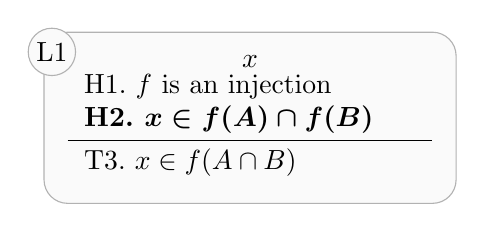
\begin{tikzpicture}[baseline=(main.base)]%
\node[tableau] (main) {%
$x$\\

\begin{tabular}{ll}%
H1.\ $\textrm{$f$ is an injection}$&\\
\textbf{\boldmath H2.\ $\textrm{$x\in f(A)\cap f(B)$}$\unboldmath }&\textbf{\boldmath \unboldmath }
\Bstrut\\\hline\Tstrut
T3.\ $\textrm{$x\in f(A\cap B)$}$&
\end{tabular}%
};%
\node[tableaulabel] at (main.north west) [xshift=4mm, yshift=-5.5mm] {L1};
\end{tikzpicture}%
\end{fit}
\smallskip

\noindent3. Quantifier-free expansion of hypothesis H2.\nopagebreak[4] 
\marginpar{Since $x\in f(A)\cap f(B)$, $x\in f(A)$ and $x\in f(B)$.}\nopagebreak[4] 
\smallskip\nopagebreak[4] 

\begin{fit}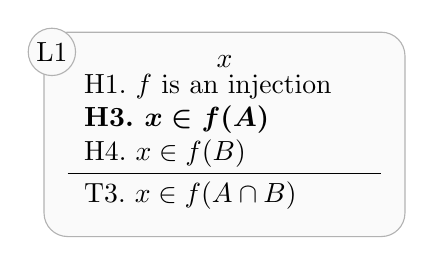
\begin{tikzpicture}[baseline=(main.base)]%
\node[tableau] (main) {%
$x$\\

\begin{tabular}{ll}%
H1.\ $\textrm{$f$ is an injection}$&\\
\textbf{\boldmath H3.\ $\textrm{$x\in f(A)$}$\unboldmath }&\textbf{\boldmath \unboldmath }\\
H4.\ $\textrm{$x\in f(B)$}$&
\Bstrut\\\hline\Tstrut
T3.\ $\textrm{$x\in f(A\cap B)$}$&
\end{tabular}%
};%
\node[tableaulabel] at (main.north west) [xshift=4mm, yshift=-5.5mm] {L1};
\end{tikzpicture}%
\end{fit}
\smallskip

\noindent4. Expand pre-existential hypothesis H3.\nopagebreak[4] 
\marginpar{By definition, since $x\in f(A)$, there exists $y\in A$ such that $f(y) = x$.}\nopagebreak[4] 
\smallskip\nopagebreak[4] 

\begin{fit}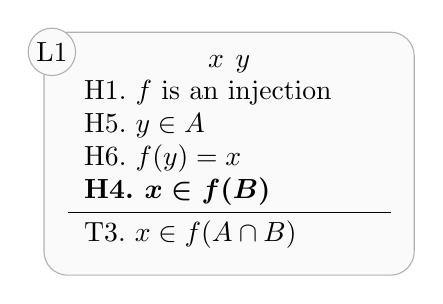
\begin{tikzpicture}[baseline=(main.base)]%
\node[tableau] (main) {%
$x$\hspace{1.5mm}$y$\\

\begin{tabular}{ll}%
H1.\ $\textrm{$f$ is an injection}$&\\
H5.\ $\textrm{$y\in A$}$&\\
H6.\ $\textrm{$f(y) = x$}$&\\
\textbf{\boldmath H4.\ $\textrm{$x\in f(B)$}$\unboldmath }&\textbf{\boldmath \unboldmath }
\Bstrut\\\hline\Tstrut
T3.\ $\textrm{$x\in f(A\cap B)$}$&
\end{tabular}%
};%
\node[tableaulabel] at (main.north west) [xshift=4mm, yshift=-5.5mm] {L1};
\end{tikzpicture}%
\end{fit}
\smallskip

\noindent5. Expand pre-existential hypothesis H4.\nopagebreak[4] 
\marginpar{By definition, since $x\in f(B)$, there exists $z\in B$ such that $f(z) = x$.}\nopagebreak[4] 
\smallskip\nopagebreak[4] 

\begin{fit}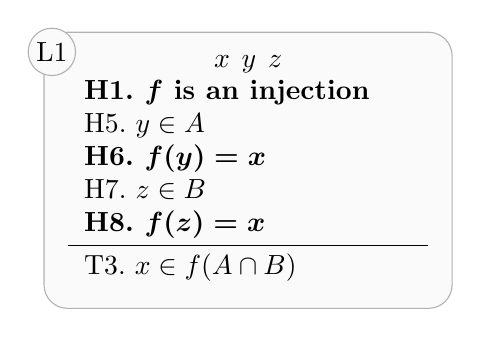
\begin{tikzpicture}[baseline=(main.base)]%
\node[tableau] (main) {%
$x$\hspace{1.5mm}$y$\hspace{1.5mm}$z$\\

\begin{tabular}{ll}%
\textbf{\boldmath H1.\ $\textrm{$f$ is an injection}$\unboldmath }&\textbf{\boldmath \unboldmath }\\
H5.\ $\textrm{$y\in A$}$&\\
\textbf{\boldmath H6.\ $\textrm{$f(y) = x$}$\unboldmath }&\textbf{\boldmath \unboldmath }\\
H7.\ $\textrm{$z\in B$}$&\\
\textbf{\boldmath H8.\ $\textrm{$f(z) = x$}$\unboldmath }&\textbf{\boldmath \unboldmath }
\Bstrut\\\hline\Tstrut
T3.\ $\textrm{$x\in f(A\cap B)$}$&
\end{tabular}%
};%
\node[tableaulabel] at (main.north west) [xshift=4mm, yshift=-5.5mm] {L1};
\end{tikzpicture}%
\end{fit}
\smallskip

\noindent6. Forwards reasoning using H1 with (H6,H8).\nopagebreak[4] 
\marginpar{Since $f$ is an injection, $f(y) = x$ and $f(z) = x$, we have that $y = z$.}\nopagebreak[4] 
\smallskip\nopagebreak[4] 

\begin{fit}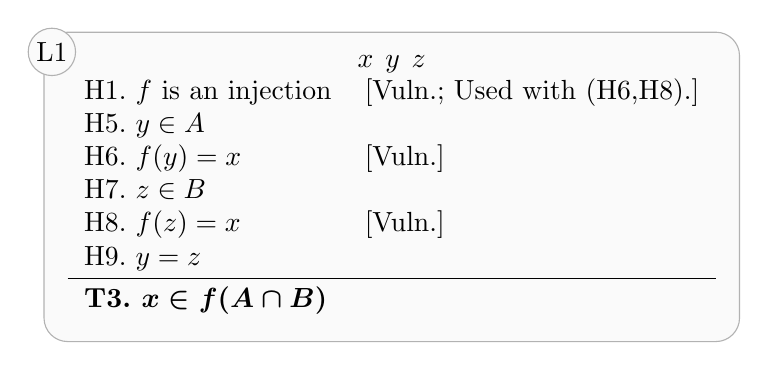
\begin{tikzpicture}[baseline=(main.base)]%
\node[tableau] (main) {%
$x$\hspace{1.5mm}$y$\hspace{1.5mm}$z$\\

\begin{tabular}{ll}%
H1.\ $\textrm{$f$ is an injection}$&[Vuln.; Used with (H6,H8).]\\
H5.\ $\textrm{$y\in A$}$&\\
H6.\ $\textrm{$f(y) = x$}$&[Vuln.]\\
H7.\ $\textrm{$z\in B$}$&\\
H8.\ $\textrm{$f(z) = x$}$&[Vuln.]\\
H9.\ $\textrm{$y = z$}$&
\Bstrut\\\hline\Tstrut
\textbf{\boldmath T3.\ $\textrm{$x\in f(A\cap B)$}$\unboldmath }&\textbf{\boldmath \unboldmath }
\end{tabular}%
};%
\node[tableaulabel] at (main.north west) [xshift=4mm, yshift=-5.5mm] {L1};
\end{tikzpicture}%
\end{fit}
\smallskip

\noindent7. Expand pre-existential target T3.\nopagebreak[4] 
\marginpar{We would like to find $u\in A\cap B$ s.t. $f(u) = x$.}\nopagebreak[4] 
\smallskip\nopagebreak[4] 

\begin{fit}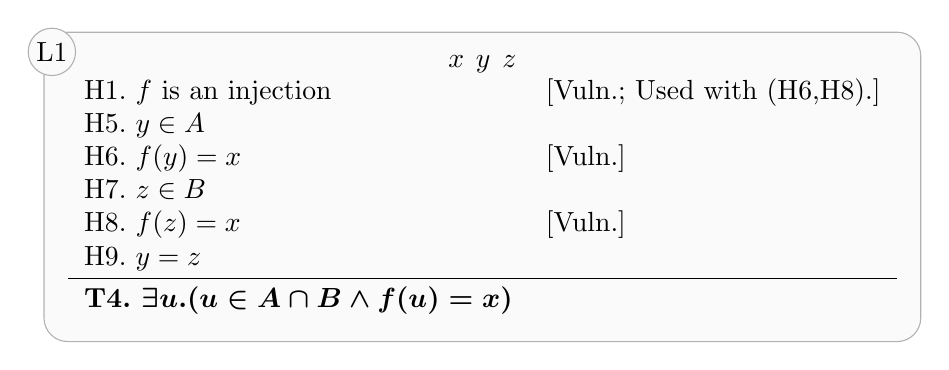
\begin{tikzpicture}[baseline=(main.base)]%
\node[tableau] (main) {%
$x$\hspace{1.5mm}$y$\hspace{1.5mm}$z$\\

\begin{tabular}{ll}%
H1.\ $\textrm{$f$ is an injection}$&[Vuln.; Used with (H6,H8).]\\
H5.\ $\textrm{$y\in A$}$&\\
H6.\ $\textrm{$f(y) = x$}$&[Vuln.]\\
H7.\ $\textrm{$z\in B$}$&\\
H8.\ $\textrm{$f(z) = x$}$&[Vuln.]\\
H9.\ $\textrm{$y = z$}$&
\Bstrut\\\hline\Tstrut
\textbf{\boldmath T4.\ $\exists u.(\textrm{$u\in A\cap B$}\wedge \textrm{$f(u) = x$})$\unboldmath }&\textbf{\boldmath \unboldmath }
\end{tabular}%
};%
\node[tableaulabel] at (main.north west) [xshift=4mm, yshift=-5.5mm] {L1};
\end{tikzpicture}%
\end{fit}
\smallskip

\noindent8. Unlock existential target T4.\nopagebreak[4] 
\marginpar{We would like to find $u\in A\cap B$ s.t. $f(u) = x$.}\nopagebreak[4] 
\smallskip\nopagebreak[4] 

\begin{fit}\begin{tikzpicture}[baseline=(main.base)]%
\node[tableau] (main) {%
$x$\hspace{1.5mm}$y$\hspace{1.5mm}$z$\\

\begin{tabular}{ll}%
H1.\ $\textrm{$f$ is an injection}$&[Vuln.; Used with (H6,H8).]\\
H5.\ $\textrm{$y\in A$}$&\\
H6.\ $\textrm{$f(y) = x$}$&[Vuln.]\\
H7.\ $\textrm{$z\in B$}$&\\
H8.\ $\textrm{$f(z) = x$}$&[Vuln.]\\
H9.\ $\textrm{$y = z$}$&
\Bstrut\\\hline\Tstrut
\begin{tikzpicture}[baseline=(main.base)]%
\node[tableau] (main) {%
$u^\blacklozenge $\\

\begin{tabular}{ll}%

\Bstrut\\\hline\Tstrut
\textbf{\boldmath T5.\ $\textrm{$u^\blacklozenge \in A\cap B$}$\unboldmath }&\textbf{\boldmath \unboldmath }\\
T6.\ $\textrm{$f(u^\blacklozenge ) = x$}$&
\end{tabular}%
};%
\node[tableaulabel] at (main.north west) [xshift=4mm, yshift=-5.5mm] {L2$^\blacklozenge$};
\end{tikzpicture}%

\end{tabular}%
};%
\node[tableaulabel] at (main.north west) [xshift=4mm, yshift=-5.5mm] {L1};
\end{tikzpicture}%
\end{fit}
\smallskip

\noindent9. Quantifier-free expansion of target T5.\nopagebreak[4] 
\marginpar{But $u\in A\cap B$ if and only if $u\in A$ and $u\in B$.}\nopagebreak[4] 
\smallskip\nopagebreak[4] 

\begin{fit}\begin{tikzpicture}[baseline=(main.base)]%
\node[tableau] (main) {%
$x$\hspace{1.5mm}$y$\hspace{1.5mm}$z$\\

\begin{tabular}{ll}%
H1.\ $\textrm{$f$ is an injection}$&[Vuln.; Used with (H6,H8).]\\
H5.\ $\textrm{$y\in A$}$&\\
H6.\ $\textrm{$f(y) = x$}$&[Vuln.]\\
H7.\ $\textrm{$z\in B$}$&\\
H8.\ $\textrm{$f(z) = x$}$&[Vuln.]\\
\textbf{\boldmath H9.\ $\textrm{$y = z$}$\unboldmath }&\textbf{\boldmath \unboldmath }
\Bstrut\\\hline\Tstrut
\begin{tikzpicture}[baseline=(main.base)]%
\node[tableau] (main) {%
$u^\blacklozenge $\\

\begin{tabular}{ll}%

\Bstrut\\\hline\Tstrut
T7.\ $\textrm{$u^\blacklozenge \in A$}$&\\
T8.\ $\textrm{$u^\blacklozenge \in B$}$&\\
T6.\ $\textrm{$f(u^\blacklozenge ) = x$}$&
\end{tabular}%
};%
\node[tableaulabel] at (main.north west) [xshift=4mm, yshift=-5.5mm] {L2$^\blacklozenge$};
\end{tikzpicture}%

\end{tabular}%
};%
\node[tableaulabel] at (main.north west) [xshift=4mm, yshift=-5.5mm] {L1};
\end{tikzpicture}%
\end{fit}
\smallskip

\noindent10. Rewrite $z$ as $y$ throughout the tableau using hypothesis H9.\nopagebreak[4] 
\marginpar{Since $y = z$, we have that $y\in B$.}\nopagebreak[4] 
\smallskip\nopagebreak[4] 

\begin{fit}\begin{tikzpicture}[baseline=(main.base)]%
\node[tableau] (main) {%
$x$\hspace{1.5mm}$y$\hspace{1.5mm}$z$\\

\begin{tabular}{ll}%
H1.\ $\textrm{$f$ is an injection}$&[Vuln.; Used with (H6,H8).]\\
H5.\ $\textrm{$y\in A$}$&\\
H6.\ $\textrm{$f(y) = x$}$&[Vuln.]\\
H10.\ $\textrm{$y\in B$}$&
\Bstrut\\\hline\Tstrut
\begin{tikzpicture}[baseline=(main.base)]%
\node[tableau] (main) {%
$u^\blacklozenge $\\

\begin{tabular}{ll}%

\Bstrut\\\hline\Tstrut
T7.\ $\textrm{$u^\blacklozenge \in A$}$&\\
T8.\ $\textrm{$u^\blacklozenge \in B$}$&\\
T6.\ $\textrm{$f(u^\blacklozenge ) = x$}$&
\end{tabular}%
};%
\node[tableaulabel] at (main.north west) [xshift=4mm, yshift=-5.5mm] {L2$^\blacklozenge$};
\end{tikzpicture}%

\end{tabular}%
};%
\node[tableaulabel] at (main.north west) [xshift=4mm, yshift=-5.5mm] {L1};
\end{tikzpicture}%
\end{fit}
\smallskip

\noindent11. Moved H6 down, as $x$ can only be utilised by T6.\nopagebreak[4] 
\marginpar{}\nopagebreak[4] 
\smallskip\nopagebreak[4] 

\begin{fit}\begin{tikzpicture}[baseline=(main.base)]%
\node[tableau] (main) {%
$x$\hspace{1.5mm}$y$\hspace{1.5mm}$z$\\

\begin{tabular}{ll}%
H1.\ $\textrm{$f$ is an injection}$&[Vuln.; Used with (H6,H8).]\\
H5.\ $\textrm{$y\in A$}$&\\
H10.\ $\textrm{$y\in B$}$&
\Bstrut\\\hline\Tstrut
\begin{tikzpicture}[baseline=(main.base)]%
\node[tableau] (main) {%
$u^\blacklozenge $\\

\begin{tabular}{ll}%

\Bstrut\\\hline\Tstrut
T7.\ $\textrm{$u^\blacklozenge \in A$}$&\\
T8.\ $\textrm{$u^\blacklozenge \in B$}$&\\
\begin{tikzpicture}[baseline=(main.base)]%
\node[tableau] (main) {%
\\

\begin{tabular}{ll}%
H6.\ $\textrm{$f(y) = x$}$&[Vuln.; From L1.]
\Bstrut\\\hline\Tstrut
T6.\ $\textrm{$f(u^\blacklozenge ) = x$}$&
\end{tabular}%
};%
\node[tableaulabel] at (main.north west) [xshift=4mm, yshift=-5.5mm] {L3};
\end{tikzpicture}%

\end{tabular}%
};%
\node[tableaulabel] at (main.north west) [xshift=4mm, yshift=-5.5mm] {L2$^\blacklozenge$};
\end{tikzpicture}%

\end{tabular}%
};%
\node[tableaulabel] at (main.north west) [xshift=4mm, yshift=-5.5mm] {L1};
\end{tikzpicture}%
\end{fit}
\smallskip

\noindent12. Choosing $u^\blacklozenge  = y$ matches all targets inside L2$^\blacklozenge$ against hypotheses, so L2$^\blacklozenge$ is done.\nopagebreak[4] 
\marginpar{Therefore, setting $u = y$, we are done.}\nopagebreak[4] 
\smallskip\nopagebreak[4] 

\begin{fit}\begin{tikzpicture}[baseline=(main.base)]%
\node[tableau] (main) {%
$x$\hspace{1.5mm}$y$\hspace{1.5mm}$z$\\

\begin{tabular}{ll}%
H1.\ $\textrm{$f$ is an injection}$&[Vuln.; Used with (H6,H8).]\\
H5.\ $\textrm{$y\in A$}$&\\
H10.\ $\textrm{$y\in B$}$&
\Bstrut\\\hline\Tstrut
\begin{tikzpicture}%
\node[tableau] (main) {%
\ \ \,Done
};%
\node[tableaulabel] at (main.north west) [xshift=4mm, yshift=-5.5mm] {L2$^\blacklozenge$};
\end{tikzpicture}%

\end{tabular}%
};%
\node[tableaulabel] at (main.north west) [xshift=4mm, yshift=-5.5mm] {L1};
\end{tikzpicture}%
\end{fit}
\smallskip

\noindent13. All targets of L1 are `Done', so L1 is itself done.\nopagebreak[4] 
\marginpar{}\nopagebreak[4] 
\smallskip\nopagebreak[4] 

\begin{fit}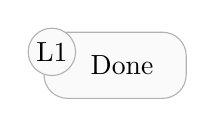
\begin{tikzpicture}%
\node[tableau] (main) {%
\ \ \,Done
};%
\node[tableaulabel] at (main.north west) [xshift=4mm, yshift=-5.5mm] {L1};
\end{tikzpicture}%
\end{fit}

Problem solved.
\cleardoublepage

\end{steps}
{\begin{center} \large \textbf{If $A$ and $B$ are open sets, then $A \cap B$ is also open.}\end{center}}\nopagebreak[4]

\begin{center}
\begin{minipage}{120mm}
Let $x$ be an element of $A\cap B$. Then $x\in A$ and $x\in B$. Therefore, since $A$ is open, there exists $\eta > 0$ such that $u\in A$\textrm{ whenever }$\textit{d}(x,u) < \eta$ and since $B$ is open, there exists $\theta > 0$ such that $v\in B$\textrm{ whenever }$\textit{d}(x,v) < \theta$. We would like to find $\delta > 0$ s.t. $y\in A\cap B$\textrm{ whenever }$\textit{d}(x,y) < \delta$. But $y\in A\cap B$ if and only if $y\in A$ and $y\in B$. We know that $y\in A$ whenever $\textit{d}(x,y) < \eta$ and that $y\in B$ whenever $\textit{d}(x,y) < \theta$. Assume now that $\textit{d}(x,y) < \delta$. Then $\textit{d}(x,y) < \eta$ if $\delta\leqslant \eta$ and $\textit{d}(x,y) < \theta$ if $\delta\leqslant \theta$. We may therefore take $\delta = \min(\eta,\theta)$ and we are done.
\end{minipage}
\end{center}

\bigskip
\begin{steps}
\begin{fit}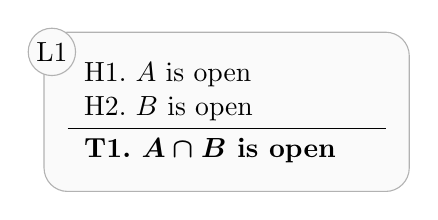
\begin{tikzpicture}[baseline=(main.base)]%
\node[tableau] (main) {%
\\

\begin{tabular}{ll}%
H1.\ $\textrm{$A$ is open}$&\\
H2.\ $\textrm{$B$ is open}$&
\Bstrut\\\hline\Tstrut
\textbf{\boldmath T1.\ $\textrm{$A\cap B$ is open}$\unboldmath }&\textbf{\boldmath \unboldmath }
\end{tabular}%
};%
\node[tableaulabel] at (main.north west) [xshift=4mm, yshift=-5.5mm] {L1};
\end{tikzpicture}%
\end{fit}
\smallskip

\noindent1. Expand pre-universal target T1.\nopagebreak[4] 
\marginpar{}\nopagebreak[4] 
\smallskip\nopagebreak[4] 

\begin{fit}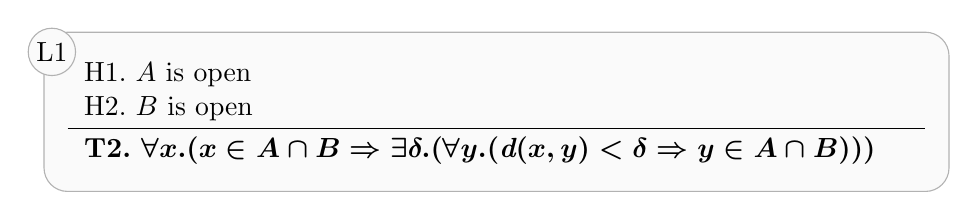
\begin{tikzpicture}[baseline=(main.base)]%
\node[tableau] (main) {%
\\

\begin{tabular}{ll}%
H1.\ $\textrm{$A$ is open}$&\\
H2.\ $\textrm{$B$ is open}$&
\Bstrut\\\hline\Tstrut
\textbf{\boldmath T2.\ $\forall x.(\textrm{$x\in A\cap B$}\Rightarrow \exists \delta.(\forall y.(\textrm{$\textit{d}(x,y) < \delta$}\Rightarrow \textrm{$y\in A\cap B$})))$\unboldmath }&\textbf{\boldmath \unboldmath }
\end{tabular}%
};%
\node[tableaulabel] at (main.north west) [xshift=4mm, yshift=-5.5mm] {L1};
\end{tikzpicture}%
\end{fit}
\smallskip

\noindent2. Apply `let' trick and move premise of universal-conditional target T2 above the line.\nopagebreak[4] 
\marginpar{Let $x$ be an element of $A\cap B$.}\nopagebreak[4] 
\smallskip\nopagebreak[4] 

\begin{fit}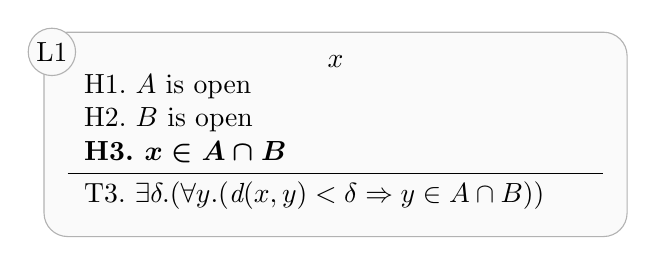
\begin{tikzpicture}[baseline=(main.base)]%
\node[tableau] (main) {%
$x$\\

\begin{tabular}{ll}%
H1.\ $\textrm{$A$ is open}$&\\
H2.\ $\textrm{$B$ is open}$&\\
\textbf{\boldmath H3.\ $\textrm{$x\in A\cap B$}$\unboldmath }&\textbf{\boldmath \unboldmath }
\Bstrut\\\hline\Tstrut
T3.\ $\exists \delta.(\forall y.(\textrm{$\textit{d}(x,y) < \delta$}\Rightarrow \textrm{$y\in A\cap B$}))$&
\end{tabular}%
};%
\node[tableaulabel] at (main.north west) [xshift=4mm, yshift=-5.5mm] {L1};
\end{tikzpicture}%
\end{fit}
\smallskip

\noindent3. Quantifier-free expansion of hypothesis H3.\nopagebreak[4] 
\marginpar{Since $x\in A\cap B$, $x\in A$ and $x\in B$.}\nopagebreak[4] 
\smallskip\nopagebreak[4] 

\begin{fit}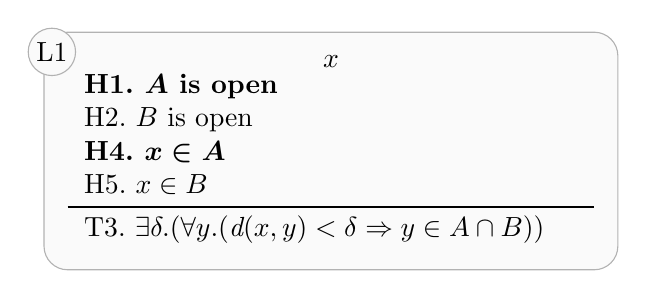
\begin{tikzpicture}[baseline=(main.base)]%
\node[tableau] (main) {%
$x$\\

\begin{tabular}{ll}%
\textbf{\boldmath H1.\ $\textrm{$A$ is open}$\unboldmath }&\textbf{\boldmath \unboldmath }\\
H2.\ $\textrm{$B$ is open}$&\\
\textbf{\boldmath H4.\ $\textrm{$x\in A$}$\unboldmath }&\textbf{\boldmath \unboldmath }\\
H5.\ $\textrm{$x\in B$}$&
\Bstrut\\\hline\Tstrut
T3.\ $\exists \delta.(\forall y.(\textrm{$\textit{d}(x,y) < \delta$}\Rightarrow \textrm{$y\in A\cap B$}))$&
\end{tabular}%
};%
\node[tableaulabel] at (main.north west) [xshift=4mm, yshift=-5.5mm] {L1};
\end{tikzpicture}%
\end{fit}
\smallskip

\noindent4. Forwards reasoning using H1 with H4.\nopagebreak[4] 
\marginpar{Since $A$ is open and $x\in A$, there exists $\eta > 0$ such that $u\in A$\textrm{ whenever }$\textit{d}(x,u) < \eta$.}\nopagebreak[4] 
\smallskip\nopagebreak[4] 

\begin{fit}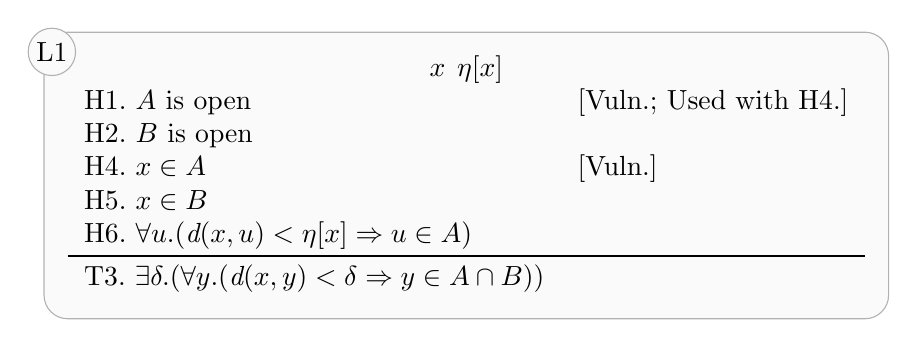
\begin{tikzpicture}[baseline=(main.base)]%
\node[tableau] (main) {%
$x$\hspace{1.5mm}$\eta[x]$\\

\begin{tabular}{ll}%
H1.\ $\textrm{$A$ is open}$&[Vuln.; Used with H4.]\\
H2.\ $\textrm{$B$ is open}$&\\
H4.\ $\textrm{$x\in A$}$&[Vuln.]\\
H5.\ $\textrm{$x\in B$}$&\\
H6.\ $\forall u.(\textrm{$\textit{d}(x,u) < \eta[x]$}\Rightarrow \textrm{$u\in A$})$&
\Bstrut\\\hline\Tstrut
T3.\ $\exists \delta.(\forall y.(\textrm{$\textit{d}(x,y) < \delta$}\Rightarrow \textrm{$y\in A\cap B$}))$&
\end{tabular}%
};%
\node[tableaulabel] at (main.north west) [xshift=4mm, yshift=-5.5mm] {L1};
\end{tikzpicture}%
\end{fit}
\smallskip

\noindent5. Deleted H4, as this unexpandable atomic statement is unmatchable.\nopagebreak[4] 
\marginpar{}\nopagebreak[4] 
\smallskip\nopagebreak[4] 

\begin{fit}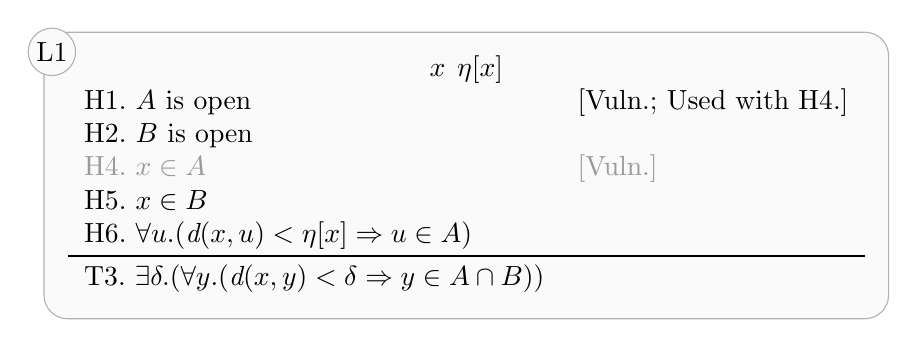
\begin{tikzpicture}[baseline=(main.base)]%
\node[tableau] (main) {%
$x$\hspace{1.5mm}$\eta[x]$\\

\begin{tabular}{ll}%
H1.\ $\textrm{$A$ is open}$&[Vuln.; Used with H4.]\\
H2.\ $\textrm{$B$ is open}$&\\
\grey{H4.\ $\textrm{$x\in A$}$}&\grey{[Vuln.]}\\
H5.\ $\textrm{$x\in B$}$&\\
H6.\ $\forall u.(\textrm{$\textit{d}(x,u) < \eta[x]$}\Rightarrow \textrm{$u\in A$})$&
\Bstrut\\\hline\Tstrut
T3.\ $\exists \delta.(\forall y.(\textrm{$\textit{d}(x,y) < \delta$}\Rightarrow \textrm{$y\in A\cap B$}))$&
\end{tabular}%
};%
\node[tableaulabel] at (main.north west) [xshift=4mm, yshift=-5.5mm] {L1};
\end{tikzpicture}%
\end{fit}
\smallskip

\noindent6. Deleted H1, as the conclusion of this implicative statement is unmatchable.\nopagebreak[4] 
\marginpar{}\nopagebreak[4] 
\smallskip\nopagebreak[4] 

\begin{fit}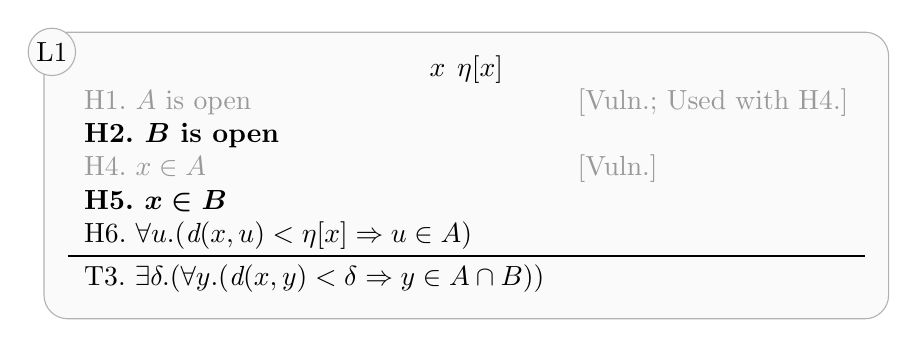
\begin{tikzpicture}[baseline=(main.base)]%
\node[tableau] (main) {%
$x$\hspace{1.5mm}$\eta[x]$\\

\begin{tabular}{ll}%
\grey{H1.\ $\textrm{$A$ is open}$}&\grey{[Vuln.; Used with H4.]}\\
\textbf{\boldmath H2.\ $\textrm{$B$ is open}$\unboldmath }&\textbf{\boldmath \unboldmath }\\
\grey{H4.\ $\textrm{$x\in A$}$}&\grey{[Vuln.]}\\
\textbf{\boldmath H5.\ $\textrm{$x\in B$}$\unboldmath }&\textbf{\boldmath \unboldmath }\\
H6.\ $\forall u.(\textrm{$\textit{d}(x,u) < \eta[x]$}\Rightarrow \textrm{$u\in A$})$&
\Bstrut\\\hline\Tstrut
T3.\ $\exists \delta.(\forall y.(\textrm{$\textit{d}(x,y) < \delta$}\Rightarrow \textrm{$y\in A\cap B$}))$&
\end{tabular}%
};%
\node[tableaulabel] at (main.north west) [xshift=4mm, yshift=-5.5mm] {L1};
\end{tikzpicture}%
\end{fit}
\smallskip

\noindent7. Forwards reasoning using H2 with H5.\nopagebreak[4] 
\marginpar{Since $B$ is open and $x\in B$, there exists $\theta > 0$ such that $v\in B$\textrm{ whenever }$\textit{d}(x,v) < \theta$.}\nopagebreak[4] 
\smallskip\nopagebreak[4] 

\begin{fit}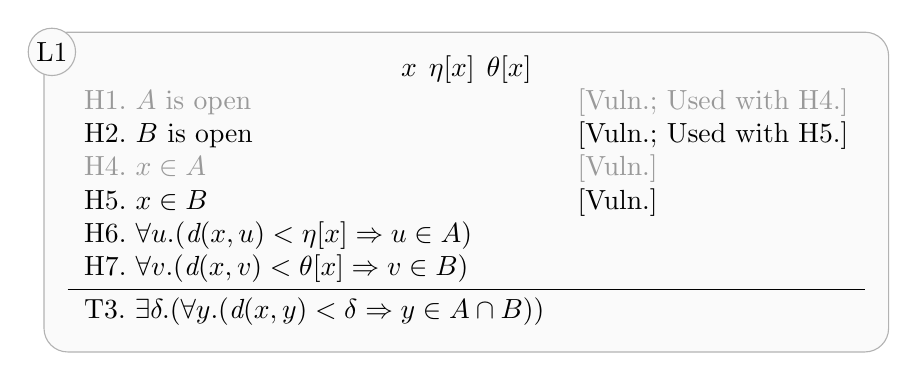
\begin{tikzpicture}[baseline=(main.base)]%
\node[tableau] (main) {%
$x$\hspace{1.5mm}$\eta[x]$\hspace{1.5mm}$\theta[x]$\\

\begin{tabular}{ll}%
\grey{H1.\ $\textrm{$A$ is open}$}&\grey{[Vuln.; Used with H4.]}\\
H2.\ $\textrm{$B$ is open}$&[Vuln.; Used with H5.]\\
\grey{H4.\ $\textrm{$x\in A$}$}&\grey{[Vuln.]}\\
H5.\ $\textrm{$x\in B$}$&[Vuln.]\\
H6.\ $\forall u.(\textrm{$\textit{d}(x,u) < \eta[x]$}\Rightarrow \textrm{$u\in A$})$&\\
H7.\ $\forall v.(\textrm{$\textit{d}(x,v) < \theta[x]$}\Rightarrow \textrm{$v\in B$})$&
\Bstrut\\\hline\Tstrut
T3.\ $\exists \delta.(\forall y.(\textrm{$\textit{d}(x,y) < \delta$}\Rightarrow \textrm{$y\in A\cap B$}))$&
\end{tabular}%
};%
\node[tableaulabel] at (main.north west) [xshift=4mm, yshift=-5.5mm] {L1};
\end{tikzpicture}%
\end{fit}
\smallskip

\noindent8. Deleted H5, as this unexpandable atomic statement is unmatchable.\nopagebreak[4] 
\marginpar{}\nopagebreak[4] 
\smallskip\nopagebreak[4] 

\begin{fit}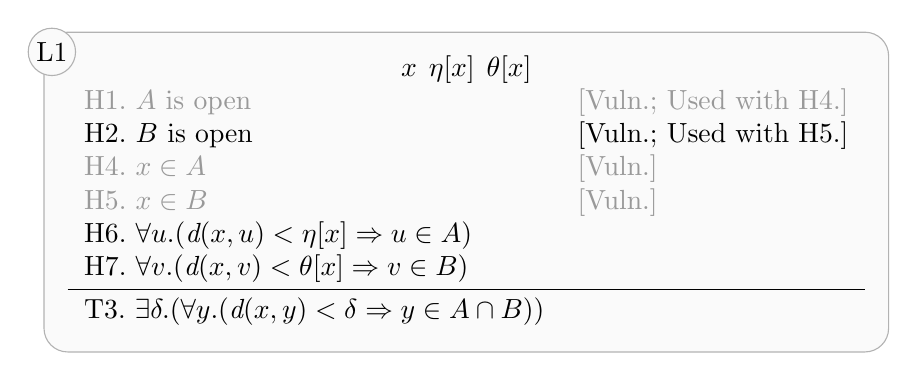
\begin{tikzpicture}[baseline=(main.base)]%
\node[tableau] (main) {%
$x$\hspace{1.5mm}$\eta[x]$\hspace{1.5mm}$\theta[x]$\\

\begin{tabular}{ll}%
\grey{H1.\ $\textrm{$A$ is open}$}&\grey{[Vuln.; Used with H4.]}\\
H2.\ $\textrm{$B$ is open}$&[Vuln.; Used with H5.]\\
\grey{H4.\ $\textrm{$x\in A$}$}&\grey{[Vuln.]}\\
\grey{H5.\ $\textrm{$x\in B$}$}&\grey{[Vuln.]}\\
H6.\ $\forall u.(\textrm{$\textit{d}(x,u) < \eta[x]$}\Rightarrow \textrm{$u\in A$})$&\\
H7.\ $\forall v.(\textrm{$\textit{d}(x,v) < \theta[x]$}\Rightarrow \textrm{$v\in B$})$&
\Bstrut\\\hline\Tstrut
T3.\ $\exists \delta.(\forall y.(\textrm{$\textit{d}(x,y) < \delta$}\Rightarrow \textrm{$y\in A\cap B$}))$&
\end{tabular}%
};%
\node[tableaulabel] at (main.north west) [xshift=4mm, yshift=-5.5mm] {L1};
\end{tikzpicture}%
\end{fit}
\smallskip

\noindent9. Deleted H2, as the conclusion of this implicative statement is unmatchable.\nopagebreak[4] 
\marginpar{}\nopagebreak[4] 
\smallskip\nopagebreak[4] 

\begin{fit}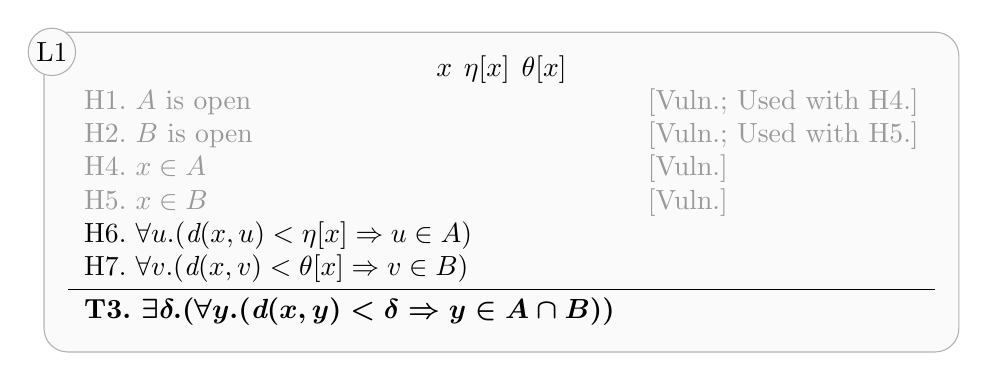
\begin{tikzpicture}[baseline=(main.base)]%
\node[tableau] (main) {%
$x$\hspace{1.5mm}$\eta[x]$\hspace{1.5mm}$\theta[x]$\\

\begin{tabular}{ll}%
\grey{H1.\ $\textrm{$A$ is open}$}&\grey{[Vuln.; Used with H4.]}\\
\grey{H2.\ $\textrm{$B$ is open}$}&\grey{[Vuln.; Used with H5.]}\\
\grey{H4.\ $\textrm{$x\in A$}$}&\grey{[Vuln.]}\\
\grey{H5.\ $\textrm{$x\in B$}$}&\grey{[Vuln.]}\\
H6.\ $\forall u.(\textrm{$\textit{d}(x,u) < \eta[x]$}\Rightarrow \textrm{$u\in A$})$&\\
H7.\ $\forall v.(\textrm{$\textit{d}(x,v) < \theta[x]$}\Rightarrow \textrm{$v\in B$})$&
\Bstrut\\\hline\Tstrut
\textbf{\boldmath T3.\ $\exists \delta.(\forall y.(\textrm{$\textit{d}(x,y) < \delta$}\Rightarrow \textrm{$y\in A\cap B$}))$\unboldmath }&\textbf{\boldmath \unboldmath }
\end{tabular}%
};%
\node[tableaulabel] at (main.north west) [xshift=4mm, yshift=-5.5mm] {L1};
\end{tikzpicture}%
\end{fit}
\smallskip

\noindent10. Unlock existential-universal-conditional target T3.\nopagebreak[4] 
\marginpar{We would like to find $\delta > 0$ s.t. $y\in A\cap B$\textrm{ whenever }$\textit{d}(x,y) < \delta$.}\nopagebreak[4] 
\smallskip\nopagebreak[4] 

\begin{fit}\begin{tikzpicture}[baseline=(main.base)]%
\node[tableau] (main) {%
$x$\hspace{1.5mm}$\eta[x]$\hspace{1.5mm}$\theta[x]$\\

\begin{tabular}{ll}%
\grey{H1.\ $\textrm{$A$ is open}$}&\grey{[Vuln.; Used with H4.]}\\
\grey{H2.\ $\textrm{$B$ is open}$}&\grey{[Vuln.; Used with H5.]}\\
\grey{H4.\ $\textrm{$x\in A$}$}&\grey{[Vuln.]}\\
\grey{H5.\ $\textrm{$x\in B$}$}&\grey{[Vuln.]}\\
H6.\ $\forall u.(\textrm{$\textit{d}(x,u) < \eta[x]$}\Rightarrow \textrm{$u\in A$})$&\\
H7.\ $\forall v.(\textrm{$\textit{d}(x,v) < \theta[x]$}\Rightarrow \textrm{$v\in B$})$&
\Bstrut\\\hline\Tstrut
\begin{tikzpicture}[baseline=(main.base)]%
\node[tableau] (main) {%
$\delta^\blacklozenge [\overline{y}]$\hspace{1.5mm}$y$\\

\begin{tabular}{ll}%
H8.\ $\textrm{$\textit{d}(x,y) < \delta^\blacklozenge [\overline{y}]$}$&[From L1.]
\Bstrut\\\hline\Tstrut
\textbf{\boldmath T4.\ $\textrm{$y\in A\cap B$}$\unboldmath }&\textbf{\boldmath \unboldmath }
\end{tabular}%
};%
\node[tableaulabel] at (main.north west) [xshift=4mm, yshift=-5.5mm] {L2$^\blacklozenge$};
\end{tikzpicture}%

\end{tabular}%
};%
\node[tableaulabel] at (main.north west) [xshift=4mm, yshift=-5.5mm] {L1};
\end{tikzpicture}%
\end{fit}
\smallskip

\noindent11. Quantifier-free expansion of target T4.\nopagebreak[4] 
\marginpar{But $y\in A\cap B$ if and only if $y\in A$ and $y\in B$.}\nopagebreak[4] 
\smallskip\nopagebreak[4] 

\begin{fit}\begin{tikzpicture}[baseline=(main.base)]%
\node[tableau] (main) {%
$x$\hspace{1.5mm}$\eta[x]$\hspace{1.5mm}$\theta[x]$\\

\begin{tabular}{ll}%
\grey{H1.\ $\textrm{$A$ is open}$}&\grey{[Vuln.; Used with H4.]}\\
\grey{H2.\ $\textrm{$B$ is open}$}&\grey{[Vuln.; Used with H5.]}\\
\grey{H4.\ $\textrm{$x\in A$}$}&\grey{[Vuln.]}\\
\grey{H5.\ $\textrm{$x\in B$}$}&\grey{[Vuln.]}\\
\textbf{\boldmath H6.\ $\forall u.(\textrm{$\textit{d}(x,u) < \eta[x]$}\Rightarrow \textrm{$u\in A$})$\unboldmath }&\textbf{\boldmath \unboldmath }\\
H7.\ $\forall v.(\textrm{$\textit{d}(x,v) < \theta[x]$}\Rightarrow \textrm{$v\in B$})$&
\Bstrut\\\hline\Tstrut
\begin{tikzpicture}[baseline=(main.base)]%
\node[tableau] (main) {%
$\delta^\blacklozenge [\overline{y}]$\hspace{1.5mm}$y$\\

\begin{tabular}{ll}%
H8.\ $\textrm{$\textit{d}(x,y) < \delta^\blacklozenge [\overline{y}]$}$&[From L1.]
\Bstrut\\\hline\Tstrut
\textbf{\boldmath T5.\ $\textrm{$y\in A$}$\unboldmath }&\textbf{\boldmath \unboldmath }\\
T6.\ $\textrm{$y\in B$}$&
\end{tabular}%
};%
\node[tableaulabel] at (main.north west) [xshift=4mm, yshift=-5.5mm] {L2$^\blacklozenge$};
\end{tikzpicture}%

\end{tabular}%
};%
\node[tableaulabel] at (main.north west) [xshift=4mm, yshift=-5.5mm] {L1};
\end{tikzpicture}%
\end{fit}
\smallskip

\noindent12. Backwards reasoning using H6 with T5.\nopagebreak[4] 
\marginpar{We know that $y\in A$ whenever $\textit{d}(x,y) < \eta$.}\nopagebreak[4] 
\smallskip\nopagebreak[4] 

\begin{fit}\begin{tikzpicture}[baseline=(main.base)]%
\node[tableau] (main) {%
$x$\hspace{1.5mm}$\eta[x]$\hspace{1.5mm}$\theta[x]$\\

\begin{tabular}{ll}%
\grey{H1.\ $\textrm{$A$ is open}$}&\grey{[Vuln.; Used with H4.]}\\
\grey{H2.\ $\textrm{$B$ is open}$}&\grey{[Vuln.; Used with H5.]}\\
\grey{H4.\ $\textrm{$x\in A$}$}&\grey{[Vuln.]}\\
\grey{H5.\ $\textrm{$x\in B$}$}&\grey{[Vuln.]}\\
H6.\ $\forall u.(\textrm{$\textit{d}(x,u) < \eta[x]$}\Rightarrow \textrm{$u\in A$})$&[Vuln.]\\
H7.\ $\forall v.(\textrm{$\textit{d}(x,v) < \theta[x]$}\Rightarrow \textrm{$v\in B$})$&
\Bstrut\\\hline\Tstrut
\begin{tikzpicture}[baseline=(main.base)]%
\node[tableau] (main) {%
$\delta^\blacklozenge [\overline{y}]$\hspace{1.5mm}$y$\\

\begin{tabular}{ll}%
H8.\ $\textrm{$\textit{d}(x,y) < \delta^\blacklozenge [\overline{y}]$}$&[From L1.]
\Bstrut\\\hline\Tstrut
T7.\ $\textrm{$\textit{d}(x,y) < \eta[x]$}$&\\
T6.\ $\textrm{$y\in B$}$&
\end{tabular}%
};%
\node[tableaulabel] at (main.north west) [xshift=4mm, yshift=-5.5mm] {L2$^\blacklozenge$};
\end{tikzpicture}%

\end{tabular}%
};%
\node[tableaulabel] at (main.north west) [xshift=4mm, yshift=-5.5mm] {L1};
\end{tikzpicture}%
\end{fit}
\smallskip

\noindent13. Delete H6 as no other statement mentions $A$.\nopagebreak[4] 
\marginpar{}\nopagebreak[4] 
\smallskip\nopagebreak[4] 

\begin{fit}\begin{tikzpicture}[baseline=(main.base)]%
\node[tableau] (main) {%
$x$\hspace{1.5mm}$\eta[x]$\hspace{1.5mm}$\theta[x]$\\

\begin{tabular}{ll}%
\grey{H1.\ $\textrm{$A$ is open}$}&\grey{[Vuln.; Used with H4.]}\\
\grey{H2.\ $\textrm{$B$ is open}$}&\grey{[Vuln.; Used with H5.]}\\
\grey{H4.\ $\textrm{$x\in A$}$}&\grey{[Vuln.]}\\
\grey{H5.\ $\textrm{$x\in B$}$}&\grey{[Vuln.]}\\
\grey{H6.\ $\forall u.(\textrm{$\textit{d}(x,u) < \eta[x]$}\Rightarrow \textrm{$u\in A$})$}&\grey{[Vuln.]}\\
\textbf{\boldmath H7.\ $\forall v.(\textrm{$\textit{d}(x,v) < \theta[x]$}\Rightarrow \textrm{$v\in B$})$\unboldmath }&\textbf{\boldmath \unboldmath }
\Bstrut\\\hline\Tstrut
\begin{tikzpicture}[baseline=(main.base)]%
\node[tableau] (main) {%
$\delta^\blacklozenge [\overline{y}]$\hspace{1.5mm}$y$\\

\begin{tabular}{ll}%
H8.\ $\textrm{$\textit{d}(x,y) < \delta^\blacklozenge [\overline{y}]$}$&[From L1.]
\Bstrut\\\hline\Tstrut
T7.\ $\textrm{$\textit{d}(x,y) < \eta[x]$}$&\\
\textbf{\boldmath T6.\ $\textrm{$y\in B$}$\unboldmath }&\textbf{\boldmath \unboldmath }
\end{tabular}%
};%
\node[tableaulabel] at (main.north west) [xshift=4mm, yshift=-5.5mm] {L2$^\blacklozenge$};
\end{tikzpicture}%

\end{tabular}%
};%
\node[tableaulabel] at (main.north west) [xshift=4mm, yshift=-5.5mm] {L1};
\end{tikzpicture}%
\end{fit}
\smallskip

\noindent14. Backwards reasoning using H7 with T6.\nopagebreak[4] 
\marginpar{We know that $y\in B$ whenever $\textit{d}(x,y) < \theta$.}\nopagebreak[4] 
\smallskip\nopagebreak[4] 

\begin{fit}\begin{tikzpicture}[baseline=(main.base)]%
\node[tableau] (main) {%
$x$\hspace{1.5mm}$\eta[x]$\hspace{1.5mm}$\theta[x]$\\

\begin{tabular}{ll}%
\grey{H1.\ $\textrm{$A$ is open}$}&\grey{[Vuln.; Used with H4.]}\\
\grey{H2.\ $\textrm{$B$ is open}$}&\grey{[Vuln.; Used with H5.]}\\
\grey{H4.\ $\textrm{$x\in A$}$}&\grey{[Vuln.]}\\
\grey{H5.\ $\textrm{$x\in B$}$}&\grey{[Vuln.]}\\
\grey{H6.\ $\forall u.(\textrm{$\textit{d}(x,u) < \eta[x]$}\Rightarrow \textrm{$u\in A$})$}&\grey{[Vuln.]}\\
H7.\ $\forall v.(\textrm{$\textit{d}(x,v) < \theta[x]$}\Rightarrow \textrm{$v\in B$})$&[Vuln.]
\Bstrut\\\hline\Tstrut
\begin{tikzpicture}[baseline=(main.base)]%
\node[tableau] (main) {%
$\delta^\blacklozenge [\overline{y}]$\hspace{1.5mm}$y$\\

\begin{tabular}{ll}%
H8.\ $\textrm{$\textit{d}(x,y) < \delta^\blacklozenge [\overline{y}]$}$&[From L1.]
\Bstrut\\\hline\Tstrut
T7.\ $\textrm{$\textit{d}(x,y) < \eta[x]$}$&\\
T8.\ $\textrm{$\textit{d}(x,y) < \theta[x]$}$&
\end{tabular}%
};%
\node[tableaulabel] at (main.north west) [xshift=4mm, yshift=-5.5mm] {L2$^\blacklozenge$};
\end{tikzpicture}%

\end{tabular}%
};%
\node[tableaulabel] at (main.north west) [xshift=4mm, yshift=-5.5mm] {L1};
\end{tikzpicture}%
\end{fit}
\smallskip

\noindent15. Delete H7 as no other statement mentions $B$.\nopagebreak[4] 
\marginpar{}\nopagebreak[4] 
\smallskip\nopagebreak[4] 

\begin{fit}\begin{tikzpicture}[baseline=(main.base)]%
\node[tableau] (main) {%
$x$\hspace{1.5mm}$\eta[x]$\hspace{1.5mm}$\theta[x]$\\

\begin{tabular}{ll}%
\grey{H1.\ $\textrm{$A$ is open}$}&\grey{[Vuln.; Used with H4.]}\\
\grey{H2.\ $\textrm{$B$ is open}$}&\grey{[Vuln.; Used with H5.]}\\
\grey{H4.\ $\textrm{$x\in A$}$}&\grey{[Vuln.]}\\
\grey{H5.\ $\textrm{$x\in B$}$}&\grey{[Vuln.]}\\
\grey{H6.\ $\forall u.(\textrm{$\textit{d}(x,u) < \eta[x]$}\Rightarrow \textrm{$u\in A$})$}&\grey{[Vuln.]}\\
\grey{H7.\ $\forall v.(\textrm{$\textit{d}(x,v) < \theta[x]$}\Rightarrow \textrm{$v\in B$})$}&\grey{[Vuln.]}
\Bstrut\\\hline\Tstrut
\begin{tikzpicture}[baseline=(main.base)]%
\node[tableau] (main) {%
$\delta^\blacklozenge [\overline{y}]$\hspace{1.5mm}$y$\\

\begin{tabular}{ll}%
H8.\ $\textrm{$\textit{d}(x,y) < \delta^\blacklozenge [\overline{y}]$}$&[From L1.]
\Bstrut\\\hline\Tstrut
T7.\ $\textrm{$\textit{d}(x,y) < \eta[x]$}$&\\
T8.\ $\textrm{$\textit{d}(x,y) < \theta[x]$}$&
\end{tabular}%
};%
\node[tableaulabel] at (main.north west) [xshift=4mm, yshift=-5.5mm] {L2$^\blacklozenge$};
\end{tikzpicture}%

\end{tabular}%
};%
\node[tableaulabel] at (main.north west) [xshift=4mm, yshift=-5.5mm] {L1};
\end{tikzpicture}%
\end{fit}
\smallskip

\noindent16. Replacing diamonds with bullets in L2$^\blacklozenge$.\nopagebreak[4] 
\marginpar{Assume now that $\textit{d}(x,y) < \delta$.}\nopagebreak[4] 
\smallskip\nopagebreak[4] 

\begin{fit}\begin{tikzpicture}[baseline=(main.base)]%
\node[tableau] (main) {%
$x$\hspace{1.5mm}$\eta[x]$\hspace{1.5mm}$\theta[x]$\\

\begin{tabular}{ll}%
\grey{H1.\ $\textrm{$A$ is open}$}&\grey{[Vuln.; Used with H4.]}\\
\grey{H2.\ $\textrm{$B$ is open}$}&\grey{[Vuln.; Used with H5.]}\\
\grey{H4.\ $\textrm{$x\in A$}$}&\grey{[Vuln.]}\\
\grey{H5.\ $\textrm{$x\in B$}$}&\grey{[Vuln.]}\\
\grey{H6.\ $\forall u.(\textrm{$\textit{d}(x,u) < \eta[x]$}\Rightarrow \textrm{$u\in A$})$}&\grey{[Vuln.]}\\
\grey{H7.\ $\forall v.(\textrm{$\textit{d}(x,v) < \theta[x]$}\Rightarrow \textrm{$v\in B$})$}&\grey{[Vuln.]}
\Bstrut\\\hline\Tstrut
\begin{tikzpicture}[baseline=(main.base)]%
\node[tableau] (main) {%
$\delta^\bullet [\overline{y}]$\hspace{1.5mm}$y$\\

\begin{tabular}{ll}%
\textbf{\boldmath H8.\ $\textrm{$\textit{d}(x,y) < \delta^\bullet [\overline{y}]$}$\unboldmath }&\textbf{\boldmath [From L1.]\unboldmath }
\Bstrut\\\hline\Tstrut
\textbf{\boldmath T7.\ $\textrm{$\textit{d}(x,y) < \eta[x]$}$\unboldmath }&\textbf{\boldmath \unboldmath }\\
T8.\ $\textrm{$\textit{d}(x,y) < \theta[x]$}$&
\end{tabular}%
};%
\node[tableaulabel] at (main.north west) [xshift=4mm, yshift=-5.5mm] {L2};
\end{tikzpicture}%

\end{tabular}%
};%
\node[tableaulabel] at (main.north west) [xshift=4mm, yshift=-5.5mm] {L1};
\end{tikzpicture}%
\end{fit}
\smallskip

\noindent17. Backwards reasoning using library result ``transitivity'' with (T7,H8).\nopagebreak[4] 
\marginpar{Since $\textit{d}(x,y) < \delta$, $\textit{d}(x,y) < \eta$ if $\delta\leqslant \eta$.}\nopagebreak[4] 
\smallskip\nopagebreak[4] 

\begin{fit}\begin{tikzpicture}[baseline=(main.base)]%
\node[tableau] (main) {%
$x$\hspace{1.5mm}$\eta[x]$\hspace{1.5mm}$\theta[x]$\\

\begin{tabular}{ll}%
\grey{H1.\ $\textrm{$A$ is open}$}&\grey{[Vuln.; Used with H4.]}\\
\grey{H2.\ $\textrm{$B$ is open}$}&\grey{[Vuln.; Used with H5.]}\\
\grey{H4.\ $\textrm{$x\in A$}$}&\grey{[Vuln.]}\\
\grey{H5.\ $\textrm{$x\in B$}$}&\grey{[Vuln.]}\\
\grey{H6.\ $\forall u.(\textrm{$\textit{d}(x,u) < \eta[x]$}\Rightarrow \textrm{$u\in A$})$}&\grey{[Vuln.]}\\
\grey{H7.\ $\forall v.(\textrm{$\textit{d}(x,v) < \theta[x]$}\Rightarrow \textrm{$v\in B$})$}&\grey{[Vuln.]}
\Bstrut\\\hline\Tstrut
\begin{tikzpicture}[baseline=(main.base)]%
\node[tableau] (main) {%
$\delta^\bullet [\overline{y}]$\hspace{1.5mm}$y$\\

\begin{tabular}{ll}%
H8.\ $\textrm{$\textit{d}(x,y) < \delta^\bullet [\overline{y}]$}$&[From L1.; Vuln.]
\Bstrut\\\hline\Tstrut
T9.\ $\textrm{$\delta^\bullet [\overline{y}]\leqslant \eta[x]$}$&\\
T8.\ $\textrm{$\textit{d}(x,y) < \theta[x]$}$&
\end{tabular}%
};%
\node[tableaulabel] at (main.north west) [xshift=4mm, yshift=-5.5mm] {L2};
\end{tikzpicture}%

\end{tabular}%
};%
\node[tableaulabel] at (main.north west) [xshift=4mm, yshift=-5.5mm] {L1};
\end{tikzpicture}%
\end{fit}
\smallskip

\noindent18. Moved H8 down, as $x$ can only be utilised by T8.\nopagebreak[4] 
\marginpar{}\nopagebreak[4] 
\smallskip\nopagebreak[4] 

\begin{fit}\begin{tikzpicture}[baseline=(main.base)]%
\node[tableau] (main) {%
$x$\hspace{1.5mm}$\eta[x]$\hspace{1.5mm}$\theta[x]$\\

\begin{tabular}{ll}%
\grey{H1.\ $\textrm{$A$ is open}$}&\grey{[Vuln.; Used with H4.]}\\
\grey{H2.\ $\textrm{$B$ is open}$}&\grey{[Vuln.; Used with H5.]}\\
\grey{H4.\ $\textrm{$x\in A$}$}&\grey{[Vuln.]}\\
\grey{H5.\ $\textrm{$x\in B$}$}&\grey{[Vuln.]}\\
\grey{H6.\ $\forall u.(\textrm{$\textit{d}(x,u) < \eta[x]$}\Rightarrow \textrm{$u\in A$})$}&\grey{[Vuln.]}\\
\grey{H7.\ $\forall v.(\textrm{$\textit{d}(x,v) < \theta[x]$}\Rightarrow \textrm{$v\in B$})$}&\grey{[Vuln.]}
\Bstrut\\\hline\Tstrut
\begin{tikzpicture}[baseline=(main.base)]%
\node[tableau] (main) {%
$\delta^\bullet [\overline{y}]$\hspace{1.5mm}$y$\\

\begin{tabular}{ll}%

\Bstrut\\\hline\Tstrut
T9.\ $\textrm{$\delta^\bullet [\overline{y}]\leqslant \eta[x]$}$&\\
\begin{tikzpicture}[baseline=(main.base)]%
\node[tableau] (main) {%
\\

\begin{tabular}{ll}%
\textbf{\boldmath H8.\ $\textrm{$\textit{d}(x,y) < \delta^\bullet [\overline{y}]$}$\unboldmath }&\textbf{\boldmath [From L1.; Vuln.; From L2.]\unboldmath }
\Bstrut\\\hline\Tstrut
\textbf{\boldmath T8.\ $\textrm{$\textit{d}(x,y) < \theta[x]$}$\unboldmath }&\textbf{\boldmath \unboldmath }
\end{tabular}%
};%
\node[tableaulabel] at (main.north west) [xshift=4mm, yshift=-5.5mm] {L3};
\end{tikzpicture}%

\end{tabular}%
};%
\node[tableaulabel] at (main.north west) [xshift=4mm, yshift=-5.5mm] {L2};
\end{tikzpicture}%

\end{tabular}%
};%
\node[tableaulabel] at (main.north west) [xshift=4mm, yshift=-5.5mm] {L1};
\end{tikzpicture}%
\end{fit}
\smallskip

\noindent19. Backwards reasoning using library result ``transitivity'' with (T8,H8).\nopagebreak[4] 
\marginpar{Since $\textit{d}(x,y) < \delta$, $\textit{d}(x,y) < \theta$ if $\delta\leqslant \theta$.}\nopagebreak[4] 
\smallskip\nopagebreak[4] 

\begin{fit}\begin{tikzpicture}[baseline=(main.base)]%
\node[tableau] (main) {%
$x$\hspace{1.5mm}$\eta[x]$\hspace{1.5mm}$\theta[x]$\\

\begin{tabular}{ll}%
\grey{H1.\ $\textrm{$A$ is open}$}&\grey{[Vuln.; Used with H4.]}\\
\grey{H2.\ $\textrm{$B$ is open}$}&\grey{[Vuln.; Used with H5.]}\\
\grey{H4.\ $\textrm{$x\in A$}$}&\grey{[Vuln.]}\\
\grey{H5.\ $\textrm{$x\in B$}$}&\grey{[Vuln.]}\\
\grey{H6.\ $\forall u.(\textrm{$\textit{d}(x,u) < \eta[x]$}\Rightarrow \textrm{$u\in A$})$}&\grey{[Vuln.]}\\
\grey{H7.\ $\forall v.(\textrm{$\textit{d}(x,v) < \theta[x]$}\Rightarrow \textrm{$v\in B$})$}&\grey{[Vuln.]}
\Bstrut\\\hline\Tstrut
\begin{tikzpicture}[baseline=(main.base)]%
\node[tableau] (main) {%
$\delta^\bullet [\overline{y}]$\hspace{1.5mm}$y$\\

\begin{tabular}{ll}%

\Bstrut\\\hline\Tstrut
T9.\ $\textrm{$\delta^\bullet [\overline{y}]\leqslant \eta[x]$}$&\\
\begin{tikzpicture}[baseline=(main.base)]%
\node[tableau] (main) {%
\\

\begin{tabular}{ll}%
H8.\ $\textrm{$\textit{d}(x,y) < \delta^\bullet [\overline{y}]$}$&[From L1.; Vuln.; From L2.]
\Bstrut\\\hline\Tstrut
T10.\ $\textrm{$\delta^\bullet [\overline{y}]\leqslant \theta[x]$}$&
\end{tabular}%
};%
\node[tableaulabel] at (main.north west) [xshift=4mm, yshift=-5.5mm] {L3};
\end{tikzpicture}%

\end{tabular}%
};%
\node[tableaulabel] at (main.north west) [xshift=4mm, yshift=-5.5mm] {L2};
\end{tikzpicture}%

\end{tabular}%
};%
\node[tableaulabel] at (main.north west) [xshift=4mm, yshift=-5.5mm] {L1};
\end{tikzpicture}%
\end{fit}
\smallskip

\noindent20. Delete H8 as no other statement mentions $x$.\nopagebreak[4] 
\marginpar{}\nopagebreak[4] 
\smallskip\nopagebreak[4] 

\begin{fit}\begin{tikzpicture}[baseline=(main.base)]%
\node[tableau] (main) {%
$x$\hspace{1.5mm}$\eta[x]$\hspace{1.5mm}$\theta[x]$\\

\begin{tabular}{ll}%
\grey{H1.\ $\textrm{$A$ is open}$}&\grey{[Vuln.; Used with H4.]}\\
\grey{H2.\ $\textrm{$B$ is open}$}&\grey{[Vuln.; Used with H5.]}\\
\grey{H4.\ $\textrm{$x\in A$}$}&\grey{[Vuln.]}\\
\grey{H5.\ $\textrm{$x\in B$}$}&\grey{[Vuln.]}\\
\grey{H6.\ $\forall u.(\textrm{$\textit{d}(x,u) < \eta[x]$}\Rightarrow \textrm{$u\in A$})$}&\grey{[Vuln.]}\\
\grey{H7.\ $\forall v.(\textrm{$\textit{d}(x,v) < \theta[x]$}\Rightarrow \textrm{$v\in B$})$}&\grey{[Vuln.]}
\Bstrut\\\hline\Tstrut
\begin{tikzpicture}[baseline=(main.base)]%
\node[tableau] (main) {%
$\delta^\bullet [\overline{y}]$\hspace{1.5mm}$y$\\

\begin{tabular}{ll}%

\Bstrut\\\hline\Tstrut
T9.\ $\textrm{$\delta^\bullet [\overline{y}]\leqslant \eta[x]$}$&\\
\begin{tikzpicture}[baseline=(main.base)]%
\node[tableau] (main) {%
\\

\begin{tabular}{ll}%
\grey{H8.\ $\textrm{$\textit{d}(x,y) < \delta^\bullet [\overline{y}]$}$}&\grey{[From L1.; Vuln.; From L2.]}
\Bstrut\\\hline\Tstrut
T10.\ $\textrm{$\delta^\bullet [\overline{y}]\leqslant \theta[x]$}$&
\end{tabular}%
};%
\node[tableaulabel] at (main.north west) [xshift=4mm, yshift=-5.5mm] {L3};
\end{tikzpicture}%

\end{tabular}%
};%
\node[tableaulabel] at (main.north west) [xshift=4mm, yshift=-5.5mm] {L2};
\end{tikzpicture}%

\end{tabular}%
};%
\node[tableaulabel] at (main.north west) [xshift=4mm, yshift=-5.5mm] {L1};
\end{tikzpicture}%
\end{fit}
\smallskip

\noindent21. Collapsed subtableau L3 as it has no undeleted hypotheses.\nopagebreak[4] 
\marginpar{}\nopagebreak[4] 
\smallskip\nopagebreak[4] 

\begin{fit}\begin{tikzpicture}[baseline=(main.base)]%
\node[tableau] (main) {%
$x$\hspace{1.5mm}$\eta[x]$\hspace{1.5mm}$\theta[x]$\\

\begin{tabular}{ll}%
\grey{H1.\ $\textrm{$A$ is open}$}&\grey{[Vuln.; Used with H4.]}\\
\grey{H2.\ $\textrm{$B$ is open}$}&\grey{[Vuln.; Used with H5.]}\\
\grey{H4.\ $\textrm{$x\in A$}$}&\grey{[Vuln.]}\\
\grey{H5.\ $\textrm{$x\in B$}$}&\grey{[Vuln.]}\\
\grey{H6.\ $\forall u.(\textrm{$\textit{d}(x,u) < \eta[x]$}\Rightarrow \textrm{$u\in A$})$}&\grey{[Vuln.]}\\
\grey{H7.\ $\forall v.(\textrm{$\textit{d}(x,v) < \theta[x]$}\Rightarrow \textrm{$v\in B$})$}&\grey{[Vuln.]}
\Bstrut\\\hline\Tstrut
\begin{tikzpicture}[baseline=(main.base)]%
\node[tableau] (main) {%
$\delta^\bullet [\overline{y}]$\hspace{1.5mm}$y$\\

\begin{tabular}{ll}%

\Bstrut\\\hline\Tstrut
T9.\ $\textrm{$\delta^\bullet [\overline{y}]\leqslant \eta[x]$}$&\\
T10.\ $\textrm{$\delta^\bullet [\overline{y}]\leqslant \theta[x]$}$&
\end{tabular}%
};%
\node[tableaulabel] at (main.north west) [xshift=4mm, yshift=-5.5mm] {L2};
\end{tikzpicture}%

\end{tabular}%
};%
\node[tableaulabel] at (main.north west) [xshift=4mm, yshift=-5.5mm] {L1};
\end{tikzpicture}%
\end{fit}
\smallskip

\noindent22. Taking $\delta^\bullet [\overline{y}] = \min(\eta[x],\theta[x])$ matches all targets against a library solution, so L2 is done.\nopagebreak[4] 
\marginpar{We may therefore take $\delta = \min(\eta,\theta)$. We are done.}\nopagebreak[4] 
\smallskip\nopagebreak[4] 

\begin{fit}\begin{tikzpicture}[baseline=(main.base)]%
\node[tableau] (main) {%
$x$\hspace{1.5mm}$\eta[x]$\hspace{1.5mm}$\theta[x]$\\

\begin{tabular}{ll}%
\grey{H1.\ $\textrm{$A$ is open}$}&\grey{[Vuln.; Used with H4.]}\\
\grey{H2.\ $\textrm{$B$ is open}$}&\grey{[Vuln.; Used with H5.]}\\
\grey{H4.\ $\textrm{$x\in A$}$}&\grey{[Vuln.]}\\
\grey{H5.\ $\textrm{$x\in B$}$}&\grey{[Vuln.]}\\
\grey{H6.\ $\forall u.(\textrm{$\textit{d}(x,u) < \eta[x]$}\Rightarrow \textrm{$u\in A$})$}&\grey{[Vuln.]}\\
\grey{H7.\ $\forall v.(\textrm{$\textit{d}(x,v) < \theta[x]$}\Rightarrow \textrm{$v\in B$})$}&\grey{[Vuln.]}
\Bstrut\\\hline\Tstrut
\begin{tikzpicture}%
\node[tableau] (main) {%
\ \ \,Done
};%
\node[tableaulabel] at (main.north west) [xshift=4mm, yshift=-5.5mm] {L2};
\end{tikzpicture}%

\end{tabular}%
};%
\node[tableaulabel] at (main.north west) [xshift=4mm, yshift=-5.5mm] {L1};
\end{tikzpicture}%
\end{fit}
\smallskip

\noindent23. All targets of L1 are `Done', so L1 is itself done.\nopagebreak[4] 
\marginpar{}\nopagebreak[4] 
\smallskip\nopagebreak[4] 

\begin{fit}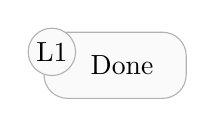
\begin{tikzpicture}%
\node[tableau] (main) {%
\ \ \,Done
};%
\node[tableaulabel] at (main.north west) [xshift=4mm, yshift=-5.5mm] {L1};
\end{tikzpicture}%
\end{fit}

Problem solved.
\cleardoublepage

\end{steps}
{\begin{center} \large \textbf{The pre-image of an open set $U$ under a continuous function $f$ is open.}\end{center}}\nopagebreak[4]

\begin{center}
\begin{minipage}{120mm}
Let $x$ be an element of $f^{-1}(U)$. Then $f(x)\in U$. Therefore, since $U$ is open, there exists $\eta > 0$ such that $u\in U$\textrm{ whenever }$\textit{d}(f(x),u) < \eta$. We would like to find $\delta > 0$ s.t. $y\in f^{-1}(U)$\textrm{ whenever }$\textit{d}(x,y) < \delta$. But $y\in f^{-1}(U)$ if and only if $f(y)\in U$. We know that $f(y)\in U$ whenever $\textit{d}(f(x),f(y)) < \eta$. Since $f$ is continuous, there exists $\theta > 0$ such that $\textit{d}(f(x),f(y)) < \eta$ whenever $\textit{d}(x,y) < \theta$. Therefore, setting $\delta = \theta$, we are done.
\end{minipage}
\end{center}

\bigskip
\begin{steps}
\begin{fit}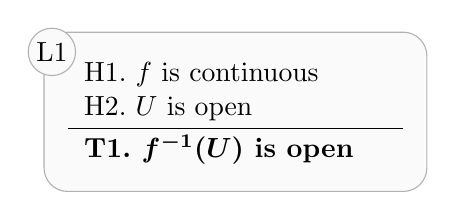
\begin{tikzpicture}[baseline=(main.base)]%
\node[tableau] (main) {%
\\

\begin{tabular}{ll}%
H1.\ $\textrm{$f$ is continuous}$&\\
H2.\ $\textrm{$U$ is open}$&
\Bstrut\\\hline\Tstrut
\textbf{\boldmath T1.\ $\textrm{$f^{-1}(U)$ is open}$\unboldmath }&\textbf{\boldmath \unboldmath }
\end{tabular}%
};%
\node[tableaulabel] at (main.north west) [xshift=4mm, yshift=-5.5mm] {L1};
\end{tikzpicture}%
\end{fit}
\smallskip

\noindent1. Expand pre-universal target T1.\nopagebreak[4] 
\marginpar{}\nopagebreak[4] 
\smallskip\nopagebreak[4] 

\begin{fit}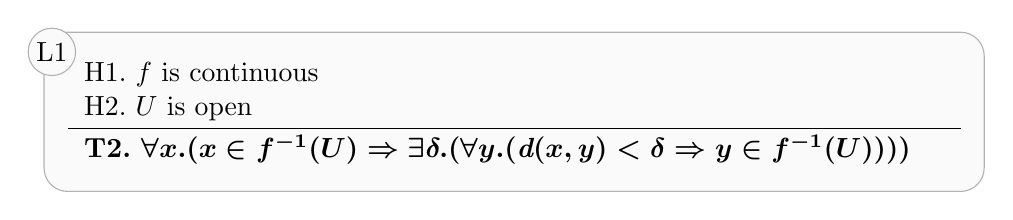
\begin{tikzpicture}[baseline=(main.base)]%
\node[tableau] (main) {%
\\

\begin{tabular}{ll}%
H1.\ $\textrm{$f$ is continuous}$&\\
H2.\ $\textrm{$U$ is open}$&
\Bstrut\\\hline\Tstrut
\textbf{\boldmath T2.\ $\forall x.(\textrm{$x\in f^{-1}(U)$}\Rightarrow \exists \delta.(\forall y.(\textrm{$\textit{d}(x,y) < \delta$}\Rightarrow \textrm{$y\in f^{-1}(U)$})))$\unboldmath }&\textbf{\boldmath \unboldmath }
\end{tabular}%
};%
\node[tableaulabel] at (main.north west) [xshift=4mm, yshift=-5.5mm] {L1};
\end{tikzpicture}%
\end{fit}
\smallskip

\noindent2. Apply `let' trick and move premise of universal-conditional target T2 above the line.\nopagebreak[4] 
\marginpar{Let $x$ be an element of $f^{-1}(U)$.}\nopagebreak[4] 
\smallskip\nopagebreak[4] 

\begin{fit}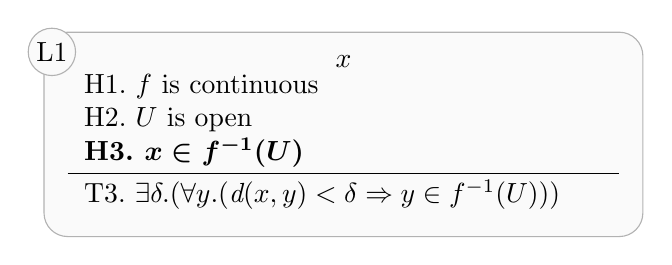
\begin{tikzpicture}[baseline=(main.base)]%
\node[tableau] (main) {%
$x$\\

\begin{tabular}{ll}%
H1.\ $\textrm{$f$ is continuous}$&\\
H2.\ $\textrm{$U$ is open}$&\\
\textbf{\boldmath H3.\ $\textrm{$x\in f^{-1}(U)$}$\unboldmath }&\textbf{\boldmath \unboldmath }
\Bstrut\\\hline\Tstrut
T3.\ $\exists \delta.(\forall y.(\textrm{$\textit{d}(x,y) < \delta$}\Rightarrow \textrm{$y\in f^{-1}(U)$}))$&
\end{tabular}%
};%
\node[tableaulabel] at (main.north west) [xshift=4mm, yshift=-5.5mm] {L1};
\end{tikzpicture}%
\end{fit}
\smallskip

\noindent3. Quantifier-free expansion of hypothesis H3.\nopagebreak[4] 
\marginpar{Since $x\in f^{-1}(U)$, we have that $f(x)\in U$.}\nopagebreak[4] 
\smallskip\nopagebreak[4] 

\begin{fit}\begin{tikzpicture}[baseline=(main.base)]%
\node[tableau] (main) {%
$x$\\

\begin{tabular}{ll}%
H1.\ $\textrm{$f$ is continuous}$&\\
\textbf{\boldmath H2.\ $\textrm{$U$ is open}$\unboldmath }&\textbf{\boldmath \unboldmath }\\
\textbf{\boldmath H4.\ $\textrm{$f(x)\in U$}$\unboldmath }&\textbf{\boldmath \unboldmath }
\Bstrut\\\hline\Tstrut
T3.\ $\exists \delta.(\forall y.(\textrm{$\textit{d}(x,y) < \delta$}\Rightarrow \textrm{$y\in f^{-1}(U)$}))$&
\end{tabular}%
};%
\node[tableaulabel] at (main.north west) [xshift=4mm, yshift=-5.5mm] {L1};
\end{tikzpicture}%
\end{fit}
\smallskip

\noindent4. Forwards reasoning using H2 with H4.\nopagebreak[4] 
\marginpar{Since $U$ is open and $f(x)\in U$, there exists $\eta > 0$ such that $u\in U$\textrm{ whenever }$\textit{d}(f(x),u) < \eta$.}\nopagebreak[4] 
\smallskip\nopagebreak[4] 

\begin{fit}\begin{tikzpicture}[baseline=(main.base)]%
\node[tableau] (main) {%
$x$\hspace{1.5mm}$\eta[f(x)]$\\

\begin{tabular}{ll}%
H1.\ $\textrm{$f$ is continuous}$&\\
H2.\ $\textrm{$U$ is open}$&[Vuln.; Used with H4.]\\
H4.\ $\textrm{$f(x)\in U$}$&[Vuln.]\\
H5.\ $\forall u.(\textrm{$\textit{d}(f(x),u) < \eta[f(x)]$}\Rightarrow \textrm{$u\in U$})$&
\Bstrut\\\hline\Tstrut
T3.\ $\exists \delta.(\forall y.(\textrm{$\textit{d}(x,y) < \delta$}\Rightarrow \textrm{$y\in f^{-1}(U)$}))$&
\end{tabular}%
};%
\node[tableaulabel] at (main.north west) [xshift=4mm, yshift=-5.5mm] {L1};
\end{tikzpicture}%
\end{fit}
\smallskip

\noindent5. Deleted H4, as this unexpandable atomic statement is unmatchable.\nopagebreak[4] 
\marginpar{}\nopagebreak[4] 
\smallskip\nopagebreak[4] 

\begin{fit}\begin{tikzpicture}[baseline=(main.base)]%
\node[tableau] (main) {%
$x$\hspace{1.5mm}$\eta[f(x)]$\\

\begin{tabular}{ll}%
H1.\ $\textrm{$f$ is continuous}$&\\
H2.\ $\textrm{$U$ is open}$&[Vuln.; Used with H4.]\\
\grey{H4.\ $\textrm{$f(x)\in U$}$}&\grey{[Vuln.]}\\
H5.\ $\forall u.(\textrm{$\textit{d}(f(x),u) < \eta[f(x)]$}\Rightarrow \textrm{$u\in U$})$&
\Bstrut\\\hline\Tstrut
T3.\ $\exists \delta.(\forall y.(\textrm{$\textit{d}(x,y) < \delta$}\Rightarrow \textrm{$y\in f^{-1}(U)$}))$&
\end{tabular}%
};%
\node[tableaulabel] at (main.north west) [xshift=4mm, yshift=-5.5mm] {L1};
\end{tikzpicture}%
\end{fit}
\smallskip

\noindent6. Deleted H2, as the conclusion of this implicative statement is unmatchable.\nopagebreak[4] 
\marginpar{}\nopagebreak[4] 
\smallskip\nopagebreak[4] 

\begin{fit}\begin{tikzpicture}[baseline=(main.base)]%
\node[tableau] (main) {%
$x$\hspace{1.5mm}$\eta[f(x)]$\\

\begin{tabular}{ll}%
H1.\ $\textrm{$f$ is continuous}$&\\
\grey{H2.\ $\textrm{$U$ is open}$}&\grey{[Vuln.; Used with H4.]}\\
\grey{H4.\ $\textrm{$f(x)\in U$}$}&\grey{[Vuln.]}\\
H5.\ $\forall u.(\textrm{$\textit{d}(f(x),u) < \eta[f(x)]$}\Rightarrow \textrm{$u\in U$})$&
\Bstrut\\\hline\Tstrut
\textbf{\boldmath T3.\ $\exists \delta.(\forall y.(\textrm{$\textit{d}(x,y) < \delta$}\Rightarrow \textrm{$y\in f^{-1}(U)$}))$\unboldmath }&\textbf{\boldmath \unboldmath }
\end{tabular}%
};%
\node[tableaulabel] at (main.north west) [xshift=4mm, yshift=-5.5mm] {L1};
\end{tikzpicture}%
\end{fit}
\smallskip

\noindent7. Unlock existential-universal-conditional target T3.\nopagebreak[4] 
\marginpar{We would like to find $\delta > 0$ s.t. $y\in f^{-1}(U)$\textrm{ whenever }$\textit{d}(x,y) < \delta$.}\nopagebreak[4] 
\smallskip\nopagebreak[4] 

\begin{fit}\begin{tikzpicture}[baseline=(main.base)]%
\node[tableau] (main) {%
$x$\hspace{1.5mm}$\eta[f(x)]$\\

\begin{tabular}{ll}%
H1.\ $\textrm{$f$ is continuous}$&\\
\grey{H2.\ $\textrm{$U$ is open}$}&\grey{[Vuln.; Used with H4.]}\\
\grey{H4.\ $\textrm{$f(x)\in U$}$}&\grey{[Vuln.]}\\
H5.\ $\forall u.(\textrm{$\textit{d}(f(x),u) < \eta[f(x)]$}\Rightarrow \textrm{$u\in U$})$&
\Bstrut\\\hline\Tstrut
\begin{tikzpicture}[baseline=(main.base)]%
\node[tableau] (main) {%
$\delta^\blacklozenge [\overline{y}]$\hspace{1.5mm}$y$\\

\begin{tabular}{ll}%
H6.\ $\textrm{$\textit{d}(x,y) < \delta^\blacklozenge [\overline{y}]$}$&[From L1.]
\Bstrut\\\hline\Tstrut
\textbf{\boldmath T4.\ $\textrm{$y\in f^{-1}(U)$}$\unboldmath }&\textbf{\boldmath \unboldmath }
\end{tabular}%
};%
\node[tableaulabel] at (main.north west) [xshift=4mm, yshift=-5.5mm] {L2$^\blacklozenge$};
\end{tikzpicture}%

\end{tabular}%
};%
\node[tableaulabel] at (main.north west) [xshift=4mm, yshift=-5.5mm] {L1};
\end{tikzpicture}%
\end{fit}
\smallskip

\noindent8. Quantifier-free expansion of target T4.\nopagebreak[4] 
\marginpar{But $y\in f^{-1}(U)$ if and only if $f(y)\in U$.}\nopagebreak[4] 
\smallskip\nopagebreak[4] 

\begin{fit}\begin{tikzpicture}[baseline=(main.base)]%
\node[tableau] (main) {%
$x$\hspace{1.5mm}$\eta[f(x)]$\\

\begin{tabular}{ll}%
H1.\ $\textrm{$f$ is continuous}$&\\
\grey{H2.\ $\textrm{$U$ is open}$}&\grey{[Vuln.; Used with H4.]}\\
\grey{H4.\ $\textrm{$f(x)\in U$}$}&\grey{[Vuln.]}\\
\textbf{\boldmath H5.\ $\forall u.(\textrm{$\textit{d}(f(x),u) < \eta[f(x)]$}\Rightarrow \textrm{$u\in U$})$\unboldmath }&\textbf{\boldmath \unboldmath }
\Bstrut\\\hline\Tstrut
\begin{tikzpicture}[baseline=(main.base)]%
\node[tableau] (main) {%
$\delta^\blacklozenge [\overline{y}]$\hspace{1.5mm}$y$\\

\begin{tabular}{ll}%
H6.\ $\textrm{$\textit{d}(x,y) < \delta^\blacklozenge [\overline{y}]$}$&[From L1.]
\Bstrut\\\hline\Tstrut
\textbf{\boldmath T5.\ $\textrm{$f(y)\in U$}$\unboldmath }&\textbf{\boldmath \unboldmath }
\end{tabular}%
};%
\node[tableaulabel] at (main.north west) [xshift=4mm, yshift=-5.5mm] {L2$^\blacklozenge$};
\end{tikzpicture}%

\end{tabular}%
};%
\node[tableaulabel] at (main.north west) [xshift=4mm, yshift=-5.5mm] {L1};
\end{tikzpicture}%
\end{fit}
\smallskip

\noindent9. Backwards reasoning using H5 with T5.\nopagebreak[4] 
\marginpar{We know that $f(y)\in U$ whenever $\textit{d}(f(x),f(y)) < \eta$.}\nopagebreak[4] 
\smallskip\nopagebreak[4] 

\begin{fit}\begin{tikzpicture}[baseline=(main.base)]%
\node[tableau] (main) {%
$x$\hspace{1.5mm}$\eta[f(x)]$\\

\begin{tabular}{ll}%
H1.\ $\textrm{$f$ is continuous}$&\\
\grey{H2.\ $\textrm{$U$ is open}$}&\grey{[Vuln.; Used with H4.]}\\
\grey{H4.\ $\textrm{$f(x)\in U$}$}&\grey{[Vuln.]}\\
H5.\ $\forall u.(\textrm{$\textit{d}(f(x),u) < \eta[f(x)]$}\Rightarrow \textrm{$u\in U$})$&[Vuln.]
\Bstrut\\\hline\Tstrut
\begin{tikzpicture}[baseline=(main.base)]%
\node[tableau] (main) {%
$\delta^\blacklozenge [\overline{y}]$\hspace{1.5mm}$y$\\

\begin{tabular}{ll}%
H6.\ $\textrm{$\textit{d}(x,y) < \delta^\blacklozenge [\overline{y}]$}$&[From L1.]
\Bstrut\\\hline\Tstrut
T6.\ $\textrm{$\textit{d}(f(x),f(y)) < \eta[f(x)]$}$&
\end{tabular}%
};%
\node[tableaulabel] at (main.north west) [xshift=4mm, yshift=-5.5mm] {L2$^\blacklozenge$};
\end{tikzpicture}%

\end{tabular}%
};%
\node[tableaulabel] at (main.north west) [xshift=4mm, yshift=-5.5mm] {L1};
\end{tikzpicture}%
\end{fit}
\smallskip

\noindent10. Delete H5 as no other statement mentions $U$.\nopagebreak[4] 
\marginpar{}\nopagebreak[4] 
\smallskip\nopagebreak[4] 

\begin{fit}\begin{tikzpicture}[baseline=(main.base)]%
\node[tableau] (main) {%
$x$\hspace{1.5mm}$\eta[f(x)]$\\

\begin{tabular}{ll}%
\textbf{\boldmath H1.\ $\textrm{$f$ is continuous}$\unboldmath }&\textbf{\boldmath \unboldmath }\\
\grey{H2.\ $\textrm{$U$ is open}$}&\grey{[Vuln.; Used with H4.]}\\
\grey{H4.\ $\textrm{$f(x)\in U$}$}&\grey{[Vuln.]}\\
\grey{H5.\ $\forall u.(\textrm{$\textit{d}(f(x),u) < \eta[f(x)]$}\Rightarrow \textrm{$u\in U$})$}&\grey{[Vuln.]}
\Bstrut\\\hline\Tstrut
\begin{tikzpicture}[baseline=(main.base)]%
\node[tableau] (main) {%
$\delta^\blacklozenge [\overline{y}]$\hspace{1.5mm}$y$\\

\begin{tabular}{ll}%
H6.\ $\textrm{$\textit{d}(x,y) < \delta^\blacklozenge [\overline{y}]$}$&[From L1.]
\Bstrut\\\hline\Tstrut
\textbf{\boldmath T6.\ $\textrm{$\textit{d}(f(x),f(y)) < \eta[f(x)]$}$\unboldmath }&\textbf{\boldmath \unboldmath }
\end{tabular}%
};%
\node[tableaulabel] at (main.north west) [xshift=4mm, yshift=-5.5mm] {L2$^\blacklozenge$};
\end{tikzpicture}%

\end{tabular}%
};%
\node[tableaulabel] at (main.north west) [xshift=4mm, yshift=-5.5mm] {L1};
\end{tikzpicture}%
\end{fit}
\smallskip

\noindent11. Backwards reasoning using H1 with T6.\nopagebreak[4] 
\marginpar{Since $f$ is continuous, there exists $\theta > 0$ such that $\textit{d}(f(x),f(y)) < \eta$ whenever $\textit{d}(x,y) < \theta$.}\nopagebreak[4] 
\smallskip\nopagebreak[4] 

\begin{fit}\begin{tikzpicture}[baseline=(main.base)]%
\node[tableau] (main) {%
$x$\hspace{1.5mm}$\eta[f(x)]$\\

\begin{tabular}{ll}%
H1.\ $\textrm{$f$ is continuous}$&[Vuln.]\\
\grey{H2.\ $\textrm{$U$ is open}$}&\grey{[Vuln.; Used with H4.]}\\
\grey{H4.\ $\textrm{$f(x)\in U$}$}&\grey{[Vuln.]}\\
\grey{H5.\ $\forall u.(\textrm{$\textit{d}(f(x),u) < \eta[f(x)]$}\Rightarrow \textrm{$u\in U$})$}&\grey{[Vuln.]}
\Bstrut\\\hline\Tstrut
\begin{tikzpicture}[baseline=(main.base)]%
\node[tableau] (main) {%
$\delta^\blacklozenge [\overline{y}]$\hspace{1.5mm}$y$\hspace{1.5mm}$\theta[z,\epsilon]$\\

\begin{tabular}{ll}%
H6.\ $\textrm{$\textit{d}(x,y) < \delta^\blacklozenge [\overline{y}]$}$&[From L1.]
\Bstrut\\\hline\Tstrut
T7.\ $\textrm{$\textit{d}(x,y) < \theta[x,\eta[f(x)]]$}$&
\end{tabular}%
};%
\node[tableaulabel] at (main.north west) [xshift=4mm, yshift=-5.5mm] {L2$^\blacklozenge$};
\end{tikzpicture}%

\end{tabular}%
};%
\node[tableaulabel] at (main.north west) [xshift=4mm, yshift=-5.5mm] {L1};
\end{tikzpicture}%
\end{fit}
\smallskip

\noindent12. Delete H1 as no other statement mentions $f$.\nopagebreak[4] 
\marginpar{}\nopagebreak[4] 
\smallskip\nopagebreak[4] 

\begin{fit}\begin{tikzpicture}[baseline=(main.base)]%
\node[tableau] (main) {%
$x$\hspace{1.5mm}$\eta[f(x)]$\\

\begin{tabular}{ll}%
\grey{H1.\ $\textrm{$f$ is continuous}$}&\grey{[Vuln.]}\\
\grey{H2.\ $\textrm{$U$ is open}$}&\grey{[Vuln.; Used with H4.]}\\
\grey{H4.\ $\textrm{$f(x)\in U$}$}&\grey{[Vuln.]}\\
\grey{H5.\ $\forall u.(\textrm{$\textit{d}(f(x),u) < \eta[f(x)]$}\Rightarrow \textrm{$u\in U$})$}&\grey{[Vuln.]}
\Bstrut\\\hline\Tstrut
\begin{tikzpicture}[baseline=(main.base)]%
\node[tableau] (main) {%
$\delta^\blacklozenge [\overline{y}]$\hspace{1.5mm}$y$\hspace{1.5mm}$\theta[z,\epsilon]$\\

\begin{tabular}{ll}%
\textbf{\boldmath H6.\ $\textrm{$\textit{d}(x,y) < \delta^\blacklozenge [\overline{y}]$}$\unboldmath }&\textbf{\boldmath [From L1.]\unboldmath }
\Bstrut\\\hline\Tstrut
\textbf{\boldmath T7.\ $\textrm{$\textit{d}(x,y) < \theta[x,\eta[f(x)]]$}$\unboldmath }&\textbf{\boldmath \unboldmath }
\end{tabular}%
};%
\node[tableaulabel] at (main.north west) [xshift=4mm, yshift=-5.5mm] {L2$^\blacklozenge$};
\end{tikzpicture}%

\end{tabular}%
};%
\node[tableaulabel] at (main.north west) [xshift=4mm, yshift=-5.5mm] {L1};
\end{tikzpicture}%
\end{fit}
\smallskip

\noindent13. Hypothesis H6 matches target T7 after choosing $\delta^\blacklozenge [\overline{y}] = \theta[x,\eta[f(x)]]$, so L2$^\blacklozenge$ is done.\nopagebreak[4] 
\marginpar{Therefore, setting $\delta = \theta$, we are done.}\nopagebreak[4] 
\smallskip\nopagebreak[4] 

\begin{fit}\begin{tikzpicture}[baseline=(main.base)]%
\node[tableau] (main) {%
$x$\hspace{1.5mm}$\eta[f(x)]$\\

\begin{tabular}{ll}%
\grey{H1.\ $\textrm{$f$ is continuous}$}&\grey{[Vuln.]}\\
\grey{H2.\ $\textrm{$U$ is open}$}&\grey{[Vuln.; Used with H4.]}\\
\grey{H4.\ $\textrm{$f(x)\in U$}$}&\grey{[Vuln.]}\\
\grey{H5.\ $\forall u.(\textrm{$\textit{d}(f(x),u) < \eta[f(x)]$}\Rightarrow \textrm{$u\in U$})$}&\grey{[Vuln.]}
\Bstrut\\\hline\Tstrut
\begin{tikzpicture}%
\node[tableau] (main) {%
\ \ \,Done
};%
\node[tableaulabel] at (main.north west) [xshift=4mm, yshift=-5.5mm] {L2$^\blacklozenge$};
\end{tikzpicture}%

\end{tabular}%
};%
\node[tableaulabel] at (main.north west) [xshift=4mm, yshift=-5.5mm] {L1};
\end{tikzpicture}%
\end{fit}
\smallskip

\noindent14. All targets of L1 are `Done', so L1 is itself done.\nopagebreak[4] 
\marginpar{}\nopagebreak[4] 
\smallskip\nopagebreak[4] 

\begin{fit}\begin{tikzpicture}%
\node[tableau] (main) {%
\ \ \,Done
};%
\node[tableaulabel] at (main.north west) [xshift=4mm, yshift=-5.5mm] {L1};
\end{tikzpicture}%
\end{fit}

Problem solved.
\cleardoublepage

\end{steps}
{\begin{center} \large \textbf{If $f$ and $g$ are continuous functions, then $g \circ f$ is continuous.}\end{center}}\nopagebreak[4]

\begin{center}
\begin{minipage}{120mm}
Take $x$ and $\epsilon > 0$. We would like to find $\delta > 0$ s.t. $\textit{d}(g(f(x)),g(f(y))) < \epsilon$\textrm{ whenever }$\textit{d}(x,y) < \delta$. Since $g$ is continuous, there exists $\eta > 0$ such that $\textit{d}(g(f(x)),g(f(y))) < \epsilon$ whenever $\textit{d}(f(x),f(y)) < \eta$. Since $f$ is continuous, there exists $\theta > 0$ such that $\textit{d}(f(x),f(y)) < \eta$ whenever $\textit{d}(x,y) < \theta$. Therefore, setting $\delta = \theta$, we are done.
\end{minipage}
\end{center}

\bigskip
\begin{steps}
\begin{fit}\begin{tikzpicture}[baseline=(main.base)]%
\node[tableau] (main) {%
\\

\begin{tabular}{ll}%
H1.\ $\textrm{$f$ is continuous}$&\\
H2.\ $\textrm{$g$ is continuous}$&
\Bstrut\\\hline\Tstrut
\textbf{\boldmath T1.\ $\textrm{$g\circ f$ is continuous}$\unboldmath }&\textbf{\boldmath \unboldmath }
\end{tabular}%
};%
\node[tableaulabel] at (main.north west) [xshift=4mm, yshift=-5.5mm] {L1};
\end{tikzpicture}%
\end{fit}
\smallskip

\noindent1. Expand pre-universal target T1.\nopagebreak[4] 
\marginpar{}\nopagebreak[4] 
\smallskip\nopagebreak[4] 

\begin{fit}\begin{tikzpicture}[baseline=(main.base)]%
\node[tableau] (main) {%
\\

\begin{tabular}{ll}%
H1.\ $\textrm{$f$ is continuous}$&\\
H2.\ $\textrm{$g$ is continuous}$&
\Bstrut\\\hline\Tstrut
\textbf{\boldmath T2.\ $\forall x, \epsilon.(\exists \delta.(\forall y.(\textrm{$\textit{d}(x,y) < \delta$}\Rightarrow \textrm{$\textit{d}(g(f(x)),g(f(y))) < \epsilon$})))$\unboldmath }&\textbf{\boldmath \unboldmath }
\end{tabular}%
};%
\node[tableaulabel] at (main.north west) [xshift=4mm, yshift=-5.5mm] {L1};
\end{tikzpicture}%
\end{fit}
\smallskip

\noindent2. pply `let' trick and move premise of universal target T2 above the line.\nopagebreak[4] 
\marginpar{Take $x$ and $\epsilon > 0$.}\nopagebreak[4] 
\smallskip\nopagebreak[4] 

\begin{fit}\begin{tikzpicture}[baseline=(main.base)]%
\node[tableau] (main) {%
$x$\hspace{1.5mm}$\epsilon$\\

\begin{tabular}{ll}%
H1.\ $\textrm{$f$ is continuous}$&\\
H2.\ $\textrm{$g$ is continuous}$&
\Bstrut\\\hline\Tstrut
\textbf{\boldmath T3.\ $\exists \delta.(\forall y.(\textrm{$\textit{d}(x,y) < \delta$}\Rightarrow \textrm{$\textit{d}(g(f(x)),g(f(y))) < \epsilon$}))$\unboldmath }&\textbf{\boldmath \unboldmath }
\end{tabular}%
};%
\node[tableaulabel] at (main.north west) [xshift=4mm, yshift=-5.5mm] {L1};
\end{tikzpicture}%
\end{fit}
\smallskip

\noindent3. Unlock existential-universal-conditional target T3.\nopagebreak[4] 
\marginpar{We would like to find $\delta > 0$ s.t. $\textit{d}(g(f(x)),g(f(y))) < \epsilon$\textrm{ whenever }$\textit{d}(x,y) < \delta$.}\nopagebreak[4] 
\smallskip\nopagebreak[4] 

\begin{fit}\begin{tikzpicture}[baseline=(main.base)]%
\node[tableau] (main) {%
$x$\hspace{1.5mm}$\epsilon$\\

\begin{tabular}{ll}%
H1.\ $\textrm{$f$ is continuous}$&\\
\textbf{\boldmath H2.\ $\textrm{$g$ is continuous}$\unboldmath }&\textbf{\boldmath \unboldmath }
\Bstrut\\\hline\Tstrut
\begin{tikzpicture}[baseline=(main.base)]%
\node[tableau] (main) {%
$\delta^\blacklozenge [\overline{y}]$\hspace{1.5mm}$y$\\

\begin{tabular}{ll}%
H3.\ $\textrm{$\textit{d}(x,y) < \delta^\blacklozenge [\overline{y}]$}$&[From L1.]
\Bstrut\\\hline\Tstrut
\textbf{\boldmath T4.\ $\textrm{$\textit{d}(g(f(x)),g(f(y))) < \epsilon$}$\unboldmath }&\textbf{\boldmath \unboldmath }
\end{tabular}%
};%
\node[tableaulabel] at (main.north west) [xshift=4mm, yshift=-5.5mm] {L2$^\blacklozenge$};
\end{tikzpicture}%

\end{tabular}%
};%
\node[tableaulabel] at (main.north west) [xshift=4mm, yshift=-5.5mm] {L1};
\end{tikzpicture}%
\end{fit}
\smallskip

\noindent4. Backwards reasoning using H2 with T4.\nopagebreak[4] 
\marginpar{Since $g$ is continuous, there exists $\eta > 0$ such that $\textit{d}(g(f(x)),g(f(y))) < \epsilon$ whenever $\textit{d}(f(x),f(y)) < \eta$.}\nopagebreak[4] 
\smallskip\nopagebreak[4] 

\begin{fit}\begin{tikzpicture}[baseline=(main.base)]%
\node[tableau] (main) {%
$x$\hspace{1.5mm}$\epsilon$\\

\begin{tabular}{ll}%
H1.\ $\textrm{$f$ is continuous}$&\\
H2.\ $\textrm{$g$ is continuous}$&[Vuln.]
\Bstrut\\\hline\Tstrut
\begin{tikzpicture}[baseline=(main.base)]%
\node[tableau] (main) {%
$\delta^\blacklozenge [\overline{y}]$\hspace{1.5mm}$y$\hspace{1.5mm}$\eta[z,\theta]$\\

\begin{tabular}{ll}%
H3.\ $\textrm{$\textit{d}(x,y) < \delta^\blacklozenge [\overline{y}]$}$&[From L1.]
\Bstrut\\\hline\Tstrut
T5.\ $\textrm{$\textit{d}(f(x),f(y)) < \eta[f(x),\epsilon]$}$&
\end{tabular}%
};%
\node[tableaulabel] at (main.north west) [xshift=4mm, yshift=-5.5mm] {L2$^\blacklozenge$};
\end{tikzpicture}%

\end{tabular}%
};%
\node[tableaulabel] at (main.north west) [xshift=4mm, yshift=-5.5mm] {L1};
\end{tikzpicture}%
\end{fit}
\smallskip

\noindent5. Delete H2 as no other statement mentions $g$.\nopagebreak[4] 
\marginpar{}\nopagebreak[4] 
\smallskip\nopagebreak[4] 

\begin{fit}\begin{tikzpicture}[baseline=(main.base)]%
\node[tableau] (main) {%
$x$\hspace{1.5mm}$\epsilon$\\

\begin{tabular}{ll}%
\textbf{\boldmath H1.\ $\textrm{$f$ is continuous}$\unboldmath }&\textbf{\boldmath \unboldmath }\\
\grey{H2.\ $\textrm{$g$ is continuous}$}&\grey{[Vuln.]}
\Bstrut\\\hline\Tstrut
\begin{tikzpicture}[baseline=(main.base)]%
\node[tableau] (main) {%
$\delta^\blacklozenge [\overline{y}]$\hspace{1.5mm}$y$\hspace{1.5mm}$\eta[z,\theta]$\\

\begin{tabular}{ll}%
H3.\ $\textrm{$\textit{d}(x,y) < \delta^\blacklozenge [\overline{y}]$}$&[From L1.]
\Bstrut\\\hline\Tstrut
\textbf{\boldmath T5.\ $\textrm{$\textit{d}(f(x),f(y)) < \eta[f(x),\epsilon]$}$\unboldmath }&\textbf{\boldmath \unboldmath }
\end{tabular}%
};%
\node[tableaulabel] at (main.north west) [xshift=4mm, yshift=-5.5mm] {L2$^\blacklozenge$};
\end{tikzpicture}%

\end{tabular}%
};%
\node[tableaulabel] at (main.north west) [xshift=4mm, yshift=-5.5mm] {L1};
\end{tikzpicture}%
\end{fit}
\smallskip

\noindent6. Backwards reasoning using H1 with T5.\nopagebreak[4] 
\marginpar{Since $f$ is continuous, there exists $\theta > 0$ such that $\textit{d}(f(x),f(y)) < \eta$ whenever $\textit{d}(x,y) < \theta$.}\nopagebreak[4] 
\smallskip\nopagebreak[4] 

\begin{fit}\begin{tikzpicture}[baseline=(main.base)]%
\node[tableau] (main) {%
$x$\hspace{1.5mm}$\epsilon$\\

\begin{tabular}{ll}%
H1.\ $\textrm{$f$ is continuous}$&[Vuln.]\\
\grey{H2.\ $\textrm{$g$ is continuous}$}&\grey{[Vuln.]}
\Bstrut\\\hline\Tstrut
\begin{tikzpicture}[baseline=(main.base)]%
\node[tableau] (main) {%
$\delta^\blacklozenge [\overline{y}]$\hspace{1.5mm}$y$\hspace{1.5mm}$\eta[z,\theta]$\hspace{1.5mm}$\theta[z,\alpha]$\\

\begin{tabular}{ll}%
H3.\ $\textrm{$\textit{d}(x,y) < \delta^\blacklozenge [\overline{y}]$}$&[From L1.]
\Bstrut\\\hline\Tstrut
T6.\ $\textrm{$\textit{d}(x,y) < \theta[x,\eta[f(x),\epsilon]]$}$&
\end{tabular}%
};%
\node[tableaulabel] at (main.north west) [xshift=4mm, yshift=-5.5mm] {L2$^\blacklozenge$};
\end{tikzpicture}%

\end{tabular}%
};%
\node[tableaulabel] at (main.north west) [xshift=4mm, yshift=-5.5mm] {L1};
\end{tikzpicture}%
\end{fit}
\smallskip

\noindent7. Delete H1 as no other statement mentions $f$.\nopagebreak[4] 
\marginpar{}\nopagebreak[4] 
\smallskip\nopagebreak[4] 

\begin{fit}\begin{tikzpicture}[baseline=(main.base)]%
\node[tableau] (main) {%
$x$\hspace{1.5mm}$\epsilon$\\

\begin{tabular}{ll}%
\grey{H1.\ $\textrm{$f$ is continuous}$}&\grey{[Vuln.]}\\
\grey{H2.\ $\textrm{$g$ is continuous}$}&\grey{[Vuln.]}
\Bstrut\\\hline\Tstrut
\begin{tikzpicture}[baseline=(main.base)]%
\node[tableau] (main) {%
$\delta^\blacklozenge [\overline{y}]$\hspace{1.5mm}$y$\hspace{1.5mm}$\eta[z,\theta]$\hspace{1.5mm}$\theta[z,\alpha]$\\

\begin{tabular}{ll}%
\textbf{\boldmath H3.\ $\textrm{$\textit{d}(x,y) < \delta^\blacklozenge [\overline{y}]$}$\unboldmath }&\textbf{\boldmath [From L1.]\unboldmath }
\Bstrut\\\hline\Tstrut
\textbf{\boldmath T6.\ $\textrm{$\textit{d}(x,y) < \theta[x,\eta[f(x),\epsilon]]$}$\unboldmath }&\textbf{\boldmath \unboldmath }
\end{tabular}%
};%
\node[tableaulabel] at (main.north west) [xshift=4mm, yshift=-5.5mm] {L2$^\blacklozenge$};
\end{tikzpicture}%

\end{tabular}%
};%
\node[tableaulabel] at (main.north west) [xshift=4mm, yshift=-5.5mm] {L1};
\end{tikzpicture}%
\end{fit}
\smallskip

\noindent8. Hypothesis H3 matches target T6 after choosing $\delta^\blacklozenge [\overline{y}] = \theta[x,\eta[f(x),\epsilon]]$, so L2$^\blacklozenge$ is done.\nopagebreak[4] 
\marginpar{Therefore, setting $\delta = \theta$, we are done.}\nopagebreak[4] 
\smallskip\nopagebreak[4] 

\begin{fit}\begin{tikzpicture}[baseline=(main.base)]%
\node[tableau] (main) {%
$x$\hspace{1.5mm}$\epsilon$\\

\begin{tabular}{ll}%
\grey{H1.\ $\textrm{$f$ is continuous}$}&\grey{[Vuln.]}\\
\grey{H2.\ $\textrm{$g$ is continuous}$}&\grey{[Vuln.]}
\Bstrut\\\hline\Tstrut
\begin{tikzpicture}%
\node[tableau] (main) {%
\ \ \,Done
};%
\node[tableaulabel] at (main.north west) [xshift=4mm, yshift=-5.5mm] {L2$^\blacklozenge$};
\end{tikzpicture}%

\end{tabular}%
};%
\node[tableaulabel] at (main.north west) [xshift=4mm, yshift=-5.5mm] {L1};
\end{tikzpicture}%
\end{fit}
\smallskip

\noindent9. All targets of L1 are `Done', so L1 is itself done.\nopagebreak[4] 
\marginpar{}\nopagebreak[4] 
\smallskip\nopagebreak[4] 

\begin{fit}\begin{tikzpicture}%
\node[tableau] (main) {%
\ \ \,Done
};%
\node[tableaulabel] at (main.north west) [xshift=4mm, yshift=-5.5mm] {L1};
\end{tikzpicture}%
\end{fit}

Problem solved.
\cleardoublepage

\end{steps}
{\begin{center} \large \textbf{If $f$ is a continuous function and $(a_n) \to a$, then $(f(a_n)) \to f(a)$}\end{center}}\nopagebreak[4]

\begin{center}
\begin{minipage}{120mm}
Let $\epsilon > 0$. We would like to find $N$ s.t. $\textit{d}(f(a),f(a_{n})) < \epsilon$\textrm{ whenever }$n\geqslant N$. Since $f$ is continuous, there exists $\delta > 0$ such that $\textit{d}(f(a),f(a_{n})) < \epsilon$ whenever $\textit{d}(a,a_{n}) < \delta$. Since $a_n\to a$, there exists $N'$ such that $\textit{d}(a,a_{n}) < \delta$ whenever $n\geqslant N'$. Therefore, setting $N = N'$, we are done.
\end{minipage}
\end{center}

\bigskip
\begin{steps}
\begin{fit}\begin{tikzpicture}[baseline=(main.base)]%
\node[tableau] (main) {%
\\

\begin{tabular}{ll}%
H1.\ $\textrm{$f$ is continuous}$&\\
H2.\ $a_n\to a$&
\Bstrut\\\hline\Tstrut
\textbf{\boldmath T1.\ $f(a_n)\to f(a)$\unboldmath }&\textbf{\boldmath \unboldmath }
\end{tabular}%
};%
\node[tableaulabel] at (main.north west) [xshift=4mm, yshift=-5.5mm] {L1};
\end{tikzpicture}%
\end{fit}
\smallskip

\noindent1. Expand pre-universal target T1.\nopagebreak[4] 
\marginpar{}\nopagebreak[4] 
\smallskip\nopagebreak[4] 

\begin{fit}\begin{tikzpicture}[baseline=(main.base)]%
\node[tableau] (main) {%
\\

\begin{tabular}{ll}%
H1.\ $\textrm{$f$ is continuous}$&\\
H2.\ $a_n\to a$&
\Bstrut\\\hline\Tstrut
\textbf{\boldmath T2.\ $\forall \epsilon.(\exists N.(\forall n.(\textrm{$n\geqslant N$}\Rightarrow \textrm{$\textit{d}(f(a),f(a_{n})) < \epsilon$})))$\unboldmath }&\textbf{\boldmath \unboldmath }
\end{tabular}%
};%
\node[tableaulabel] at (main.north west) [xshift=4mm, yshift=-5.5mm] {L1};
\end{tikzpicture}%
\end{fit}
\smallskip

\noindent2. pply `let' trick and move premise of universal target T2 above the line.\nopagebreak[4] 
\marginpar{Let $\epsilon > 0$.}\nopagebreak[4] 
\smallskip\nopagebreak[4] 

\begin{fit}\begin{tikzpicture}[baseline=(main.base)]%
\node[tableau] (main) {%
$\epsilon$\\

\begin{tabular}{ll}%
H1.\ $\textrm{$f$ is continuous}$&\\
H2.\ $a_n\to a$&
\Bstrut\\\hline\Tstrut
\textbf{\boldmath T3.\ $\exists N.(\forall n.(\textrm{$n\geqslant N$}\Rightarrow \textrm{$\textit{d}(f(a),f(a_{n})) < \epsilon$}))$\unboldmath }&\textbf{\boldmath \unboldmath }
\end{tabular}%
};%
\node[tableaulabel] at (main.north west) [xshift=4mm, yshift=-5.5mm] {L1};
\end{tikzpicture}%
\end{fit}
\smallskip

\noindent3. Unlock existential-universal-conditional target T3.\nopagebreak[4] 
\marginpar{We would like to find $N$ s.t. $\textit{d}(f(a),f(a_{n})) < \epsilon$\textrm{ whenever }$n\geqslant N$.}\nopagebreak[4] 
\smallskip\nopagebreak[4] 

\begin{fit}\begin{tikzpicture}[baseline=(main.base)]%
\node[tableau] (main) {%
$\epsilon$\\

\begin{tabular}{ll}%
\textbf{\boldmath H1.\ $\textrm{$f$ is continuous}$\unboldmath }&\textbf{\boldmath \unboldmath }\\
H2.\ $a_n\to a$&
\Bstrut\\\hline\Tstrut
\begin{tikzpicture}[baseline=(main.base)]%
\node[tableau] (main) {%
$N^\blacklozenge [\overline{n}]$\hspace{1.5mm}$n$\\

\begin{tabular}{ll}%
H3.\ $\textrm{$n\geqslant N^\blacklozenge [\overline{n}]$}$&[From L1.]
\Bstrut\\\hline\Tstrut
\textbf{\boldmath T4.\ $\textrm{$\textit{d}(f(a),f(a_{n})) < \epsilon$}$\unboldmath }&\textbf{\boldmath \unboldmath }
\end{tabular}%
};%
\node[tableaulabel] at (main.north west) [xshift=4mm, yshift=-5.5mm] {L2$^\blacklozenge$};
\end{tikzpicture}%

\end{tabular}%
};%
\node[tableaulabel] at (main.north west) [xshift=4mm, yshift=-5.5mm] {L1};
\end{tikzpicture}%
\end{fit}
\smallskip

\noindent4. Backwards reasoning using H1 with T4.\nopagebreak[4] 
\marginpar{Since $f$ is continuous, there exists $\delta > 0$ such that $\textit{d}(f(a),f(a_{n})) < \epsilon$ whenever $\textit{d}(a,a_{n}) < \delta$.}\nopagebreak[4] 
\smallskip\nopagebreak[4] 

\begin{fit}\begin{tikzpicture}[baseline=(main.base)]%
\node[tableau] (main) {%
$\epsilon$\\

\begin{tabular}{ll}%
H1.\ $\textrm{$f$ is continuous}$&[Vuln.]\\
H2.\ $a_n\to a$&
\Bstrut\\\hline\Tstrut
\begin{tikzpicture}[baseline=(main.base)]%
\node[tableau] (main) {%
$N^\blacklozenge [\overline{n}]$\hspace{1.5mm}$n$\hspace{1.5mm}$\delta[x,\eta]$\\

\begin{tabular}{ll}%
H3.\ $\textrm{$n\geqslant N^\blacklozenge [\overline{n}]$}$&[From L1.]
\Bstrut\\\hline\Tstrut
T5.\ $\textrm{$\textit{d}(a,a_{n}) < \delta[a,\epsilon]$}$&
\end{tabular}%
};%
\node[tableaulabel] at (main.north west) [xshift=4mm, yshift=-5.5mm] {L2$^\blacklozenge$};
\end{tikzpicture}%

\end{tabular}%
};%
\node[tableaulabel] at (main.north west) [xshift=4mm, yshift=-5.5mm] {L1};
\end{tikzpicture}%
\end{fit}
\smallskip

\noindent5. Delete H1 as no other statement mentions $f$.\nopagebreak[4] 
\marginpar{}\nopagebreak[4] 
\smallskip\nopagebreak[4] 

\begin{fit}\begin{tikzpicture}[baseline=(main.base)]%
\node[tableau] (main) {%
$\epsilon$\\

\begin{tabular}{ll}%
\grey{H1.\ $\textrm{$f$ is continuous}$}&\grey{[Vuln.]}\\
\textbf{\boldmath H2.\ $a_n\to a$\unboldmath }&\textbf{\boldmath \unboldmath }
\Bstrut\\\hline\Tstrut
\begin{tikzpicture}[baseline=(main.base)]%
\node[tableau] (main) {%
$N^\blacklozenge [\overline{n}]$\hspace{1.5mm}$n$\hspace{1.5mm}$\delta[x,\eta]$\\

\begin{tabular}{ll}%
H3.\ $\textrm{$n\geqslant N^\blacklozenge [\overline{n}]$}$&[From L1.]
\Bstrut\\\hline\Tstrut
\textbf{\boldmath T5.\ $\textrm{$\textit{d}(a,a_{n}) < \delta[a,\epsilon]$}$\unboldmath }&\textbf{\boldmath \unboldmath }
\end{tabular}%
};%
\node[tableaulabel] at (main.north west) [xshift=4mm, yshift=-5.5mm] {L2$^\blacklozenge$};
\end{tikzpicture}%

\end{tabular}%
};%
\node[tableaulabel] at (main.north west) [xshift=4mm, yshift=-5.5mm] {L1};
\end{tikzpicture}%
\end{fit}
\smallskip

\noindent6. Backwards reasoning using H2 with T5.\nopagebreak[4] 
\marginpar{Since $a_n\to a$, there exists $N'$ such that $\textit{d}(a,a_{n}) < \delta$ whenever $n\geqslant N'$.}\nopagebreak[4] 
\smallskip\nopagebreak[4] 

\begin{fit}\begin{tikzpicture}[baseline=(main.base)]%
\node[tableau] (main) {%
$\epsilon$\\

\begin{tabular}{ll}%
\grey{H1.\ $\textrm{$f$ is continuous}$}&\grey{[Vuln.]}\\
H2.\ $a_n\to a$&[Vuln.]
\Bstrut\\\hline\Tstrut
\begin{tikzpicture}[baseline=(main.base)]%
\node[tableau] (main) {%
$N^\blacklozenge [\overline{n}]$\hspace{1.5mm}$n$\hspace{1.5mm}$\delta[x,\eta]$\hspace{1.5mm}$N'[\eta]$\\

\begin{tabular}{ll}%
H3.\ $\textrm{$n\geqslant N^\blacklozenge [\overline{n}]$}$&[From L1.]
\Bstrut\\\hline\Tstrut
T6.\ $\textrm{$n\geqslant N'[\delta[a,\epsilon]]$}$&
\end{tabular}%
};%
\node[tableaulabel] at (main.north west) [xshift=4mm, yshift=-5.5mm] {L2$^\blacklozenge$};
\end{tikzpicture}%

\end{tabular}%
};%
\node[tableaulabel] at (main.north west) [xshift=4mm, yshift=-5.5mm] {L1};
\end{tikzpicture}%
\end{fit}
\smallskip

\noindent7. Delete H2 as no other statement mentions $a$.\nopagebreak[4] 
\marginpar{}\nopagebreak[4] 
\smallskip\nopagebreak[4] 

\begin{fit}\begin{tikzpicture}[baseline=(main.base)]%
\node[tableau] (main) {%
$\epsilon$\\

\begin{tabular}{ll}%
\grey{H1.\ $\textrm{$f$ is continuous}$}&\grey{[Vuln.]}\\
\grey{H2.\ $a_n\to a$}&\grey{[Vuln.]}
\Bstrut\\\hline\Tstrut
\begin{tikzpicture}[baseline=(main.base)]%
\node[tableau] (main) {%
$N^\blacklozenge [\overline{n}]$\hspace{1.5mm}$n$\hspace{1.5mm}$\delta[x,\eta]$\hspace{1.5mm}$N'[\eta]$\\

\begin{tabular}{ll}%
\textbf{\boldmath H3.\ $\textrm{$n\geqslant N^\blacklozenge [\overline{n}]$}$\unboldmath }&\textbf{\boldmath [From L1.]\unboldmath }
\Bstrut\\\hline\Tstrut
\textbf{\boldmath T6.\ $\textrm{$n\geqslant N'[\delta[a,\epsilon]]$}$\unboldmath }&\textbf{\boldmath \unboldmath }
\end{tabular}%
};%
\node[tableaulabel] at (main.north west) [xshift=4mm, yshift=-5.5mm] {L2$^\blacklozenge$};
\end{tikzpicture}%

\end{tabular}%
};%
\node[tableaulabel] at (main.north west) [xshift=4mm, yshift=-5.5mm] {L1};
\end{tikzpicture}%
\end{fit}
\smallskip

\noindent8. Hypothesis H3 matches target T6 after choosing $N^\blacklozenge [\overline{n}] = N'[\delta[a,\epsilon]]$, so L2$^\blacklozenge$ is done.\nopagebreak[4] 
\marginpar{Therefore, setting $N = N'$, we are done.}\nopagebreak[4] 
\smallskip\nopagebreak[4] 

\begin{fit}\begin{tikzpicture}[baseline=(main.base)]%
\node[tableau] (main) {%
$\epsilon$\\

\begin{tabular}{ll}%
\grey{H1.\ $\textrm{$f$ is continuous}$}&\grey{[Vuln.]}\\
\grey{H2.\ $a_n\to a$}&\grey{[Vuln.]}
\Bstrut\\\hline\Tstrut
\begin{tikzpicture}%
\node[tableau] (main) {%
\ \ \,Done
};%
\node[tableaulabel] at (main.north west) [xshift=4mm, yshift=-5.5mm] {L2$^\blacklozenge$};
\end{tikzpicture}%

\end{tabular}%
};%
\node[tableaulabel] at (main.north west) [xshift=4mm, yshift=-5.5mm] {L1};
\end{tikzpicture}%
\end{fit}
\smallskip

\noindent9. All targets of L1 are `Done', so L1 is itself done.\nopagebreak[4] 
\marginpar{}\nopagebreak[4] 
\smallskip\nopagebreak[4] 

\begin{fit}\begin{tikzpicture}%
\node[tableau] (main) {%
\ \ \,Done
};%
\node[tableaulabel] at (main.north west) [xshift=4mm, yshift=-5.5mm] {L1};
\end{tikzpicture}%
\end{fit}

Problem solved.
\cleardoublepage

\end{steps}
{\begin{center} \large \textbf{A closed subset $A$ of a complete metric space $X$ is complete.}\end{center}}\nopagebreak[4]

\begin{center}
\begin{minipage}{120mm}
Let $(a_n)$ be a Cauchy sequence in $A$. Then, since $X$ is complete, we have that $(a_n)$ converges. That is, there exists $a$ such that $a_n\to a$. Since $A$ is closed in $X$, $(a_n)$ is a sequence in $A$ and $a_n\to a$, we have that $a\in A$. Thus $(a_n)$ converges in $A$ and we are done.
\end{minipage}
\end{center}

\bigskip
\begin{steps}
\begin{fit}\begin{tikzpicture}[baseline=(main.base)]%
\node[tableau] (main) {%
\\

\begin{tabular}{ll}%
H1.\ $\textrm{$X$ is complete}$&\\
H2.\ $\textrm{$A$ is closed in $X$}$&
\Bstrut\\\hline\Tstrut
\textbf{\boldmath T1.\ $\textrm{$A$ is a complete space}$\unboldmath }&\textbf{\boldmath \unboldmath }
\end{tabular}%
};%
\node[tableaulabel] at (main.north west) [xshift=4mm, yshift=-5.5mm] {L1};
\end{tikzpicture}%
\end{fit}
\smallskip

\noindent1. Expand pre-universal target T1.\nopagebreak[4] 
\marginpar{}\nopagebreak[4] 
\smallskip\nopagebreak[4] 

\begin{fit}\begin{tikzpicture}[baseline=(main.base)]%
\node[tableau] (main) {%
\\

\begin{tabular}{ll}%
H1.\ $\textrm{$X$ is complete}$&\\
H2.\ $\textrm{$A$ is closed in $X$}$&
\Bstrut\\\hline\Tstrut
\textbf{\boldmath T2.\ $\forall (a_n).(\textrm{$(a_n)$ is Cauchy}\wedge \textrm{$(a_n)$ is a sequence in $A$}\Rightarrow \textrm{$(a_n)$ converges in $A$})$\unboldmath }&\textbf{\boldmath \unboldmath }
\end{tabular}%
};%
\node[tableaulabel] at (main.north west) [xshift=4mm, yshift=-5.5mm] {L1};
\end{tikzpicture}%
\end{fit}
\smallskip

\noindent2. Apply `let' trick and move premise of universal-conditional target T2 above the line.\nopagebreak[4] 
\marginpar{Let $(a_n)$ be a Cauchy sequence in $A$.}\nopagebreak[4] 
\smallskip\nopagebreak[4] 

\begin{fit}\begin{tikzpicture}[baseline=(main.base)]%
\node[tableau] (main) {%
$(a_n)$\\

\begin{tabular}{ll}%
\textbf{\boldmath H1.\ $\textrm{$X$ is complete}$\unboldmath }&\textbf{\boldmath \unboldmath }\\
H2.\ $\textrm{$A$ is closed in $X$}$&\\
\textbf{\boldmath H3.\ $\textrm{$(a_n)$ is Cauchy}$\unboldmath }&\textbf{\boldmath \unboldmath }\\
H4.\ $\textrm{$(a_n)$ is a sequence in $A$}$&
\Bstrut\\\hline\Tstrut
T3.\ $\textrm{$(a_n)$ converges in $A$}$&
\end{tabular}%
};%
\node[tableaulabel] at (main.north west) [xshift=4mm, yshift=-5.5mm] {L1};
\end{tikzpicture}%
\end{fit}
\smallskip

\noindent3. Forwards reasoning using H1 with H3.\nopagebreak[4] 
\marginpar{Since $X$ is complete and $(a_n)$ is Cauchy, we have that $(a_n)$ converges.}\nopagebreak[4] 
\smallskip\nopagebreak[4] 

\begin{fit}\begin{tikzpicture}[baseline=(main.base)]%
\node[tableau] (main) {%
$(a_n)$\\

\begin{tabular}{ll}%
H1.\ $\textrm{$X$ is complete}$&[Vuln.; Used with H3.]\\
H2.\ $\textrm{$A$ is closed in $X$}$&\\
H3.\ $\textrm{$(a_n)$ is Cauchy}$&[Vuln.]\\
H4.\ $\textrm{$(a_n)$ is a sequence in $A$}$&\\
H5.\ $\textrm{$(a_n)$ converges}$&
\Bstrut\\\hline\Tstrut
T3.\ $\textrm{$(a_n)$ converges in $A$}$&
\end{tabular}%
};%
\node[tableaulabel] at (main.north west) [xshift=4mm, yshift=-5.5mm] {L1};
\end{tikzpicture}%
\end{fit}
\smallskip

\noindent4. Deleted H1, as the conclusion of this implicative statement is unmatchable.\nopagebreak[4] 
\marginpar{}\nopagebreak[4] 
\smallskip\nopagebreak[4] 

\begin{fit}\begin{tikzpicture}[baseline=(main.base)]%
\node[tableau] (main) {%
$(a_n)$\\

\begin{tabular}{ll}%
\grey{H1.\ $\textrm{$X$ is complete}$}&\grey{[Vuln.; Used with H3.]}\\
H2.\ $\textrm{$A$ is closed in $X$}$&\\
H3.\ $\textrm{$(a_n)$ is Cauchy}$&[Vuln.]\\
H4.\ $\textrm{$(a_n)$ is a sequence in $A$}$&\\
\textbf{\boldmath H5.\ $\textrm{$(a_n)$ converges}$\unboldmath }&\textbf{\boldmath \unboldmath }
\Bstrut\\\hline\Tstrut
T3.\ $\textrm{$(a_n)$ converges in $A$}$&
\end{tabular}%
};%
\node[tableaulabel] at (main.north west) [xshift=4mm, yshift=-5.5mm] {L1};
\end{tikzpicture}%
\end{fit}
\smallskip

\noindent5. Expand pre-existential hypothesis H5.\nopagebreak[4] 
\marginpar{By definition, since $(a_n)$ converges, there exists $a$ such that $a_n\to a$.}\nopagebreak[4] 
\smallskip\nopagebreak[4] 

\begin{fit}\begin{tikzpicture}[baseline=(main.base)]%
\node[tableau] (main) {%
$(a_n)$\hspace{1.5mm}$a$\\

\begin{tabular}{ll}%
\grey{H1.\ $\textrm{$X$ is complete}$}&\grey{[Vuln.; Used with H3.]}\\
\textbf{\boldmath H2.\ $\textrm{$A$ is closed in $X$}$\unboldmath }&\textbf{\boldmath \unboldmath }\\
H3.\ $\textrm{$(a_n)$ is Cauchy}$&[Vuln.]\\
\textbf{\boldmath H4.\ $\textrm{$(a_n)$ is a sequence in $A$}$\unboldmath }&\textbf{\boldmath \unboldmath }\\
\textbf{\boldmath H6.\ $a_n\to a$\unboldmath }&\textbf{\boldmath \unboldmath }
\Bstrut\\\hline\Tstrut
T3.\ $\textrm{$(a_n)$ converges in $A$}$&
\end{tabular}%
};%
\node[tableaulabel] at (main.north west) [xshift=4mm, yshift=-5.5mm] {L1};
\end{tikzpicture}%
\end{fit}
\smallskip

\noindent6. Forwards reasoning using library result ``a closed set contains its limit points'' with (H2,H4,H6).\nopagebreak[4] 
\marginpar{Since $A$ is closed in $X$, $(a_n)$ is a sequence in $A$ and $a_n\to a$, we have that $a\in A$.}\nopagebreak[4] 
\smallskip\nopagebreak[4] 

\begin{fit}\begin{tikzpicture}[baseline=(main.base)]%
\node[tableau] (main) {%
$(a_n)$\hspace{1.5mm}$a$\\

\begin{tabular}{ll}%
\grey{H1.\ $\textrm{$X$ is complete}$}&\grey{[Vuln.; Used with H3.]}\\
H2.\ $\textrm{$A$ is closed in $X$}$&[Vuln.]\\
H3.\ $\textrm{$(a_n)$ is Cauchy}$&[Vuln.]\\
H4.\ $\textrm{$(a_n)$ is a sequence in $A$}$&[Vuln.]\\
H6.\ $a_n\to a$&[Vuln.]\\
H7.\ $\textrm{$a\in A$}$&
\Bstrut\\\hline\Tstrut
T3.\ $\textrm{$(a_n)$ converges in $A$}$&
\end{tabular}%
};%
\node[tableaulabel] at (main.north west) [xshift=4mm, yshift=-5.5mm] {L1};
\end{tikzpicture}%
\end{fit}
\smallskip

\noindent7. Delete H2 as no other statement mentions $X$.\nopagebreak[4] 
\marginpar{}\nopagebreak[4] 
\smallskip\nopagebreak[4] 

\begin{fit}\begin{tikzpicture}[baseline=(main.base)]%
\node[tableau] (main) {%
$(a_n)$\hspace{1.5mm}$a$\\

\begin{tabular}{ll}%
\grey{H1.\ $\textrm{$X$ is complete}$}&\grey{[Vuln.; Used with H3.]}\\
\grey{H2.\ $\textrm{$A$ is closed in $X$}$}&\grey{[Vuln.]}\\
H3.\ $\textrm{$(a_n)$ is Cauchy}$&[Vuln.]\\
H4.\ $\textrm{$(a_n)$ is a sequence in $A$}$&[Vuln.]\\
\textbf{\boldmath H6.\ $a_n\to a$\unboldmath }&\textbf{\boldmath [Vuln.]\unboldmath }\\
\textbf{\boldmath H7.\ $\textrm{$a\in A$}$\unboldmath }&\textbf{\boldmath \unboldmath }
\Bstrut\\\hline\Tstrut
\textbf{\boldmath T3.\ $\textrm{$(a_n)$ converges in $A$}$\unboldmath }&\textbf{\boldmath \unboldmath }
\end{tabular}%
};%
\node[tableaulabel] at (main.north west) [xshift=4mm, yshift=-5.5mm] {L1};
\end{tikzpicture}%
\end{fit}
\smallskip

\noindent8. All conjuncts of T3 (after expansion) can be simultaneously matched against H7 and H6 or rendered trivial by choosing $z = a$, so L1 is done.\nopagebreak[4] 
\marginpar{We would like to show that $(a_n)$ converges in $A$. But this is clearly the case, so we are done.}\nopagebreak[4] 
\smallskip\nopagebreak[4] 

\begin{fit}\begin{tikzpicture}%
\node[tableau] (main) {%
\ \ \,Done
};%
\node[tableaulabel] at (main.north west) [xshift=4mm, yshift=-5.5mm] {L1};
\end{tikzpicture}%
\end{fit}

Problem solved.
\cleardoublepage

\end{steps}
{\begin{center} \large \textbf{$f(f^{-1}(A))\subset A$}\end{center}}\nopagebreak[4]

\begin{center}
\begin{minipage}{120mm}
Let $x$ be an element of $f(f^{-1}(A))$. Then there exists $y\in f^{-1}(A)$ such that $f(y) = x$. Since $y\in f^{-1}(A)$, we have that $f(y)\in A$. Since $f(y) = x$, we have that $x\in A$ and we are done.
\end{minipage}
\end{center}

\bigskip
\begin{steps}
\begin{fit}\begin{tikzpicture}[baseline=(main.base)]%
\node[tableau] (main) {%
\\

\begin{tabular}{ll}%

\Bstrut\\\hline\Tstrut
\textbf{\boldmath T1.\ $\textrm{$f(f^{-1}(A))\subset A$}$\unboldmath }&\textbf{\boldmath \unboldmath }
\end{tabular}%
};%
\node[tableaulabel] at (main.north west) [xshift=4mm, yshift=-5.5mm] {L1};
\end{tikzpicture}%
\end{fit}
\smallskip

\noindent1. Expand pre-universal target T1.\nopagebreak[4] 
\marginpar{}\nopagebreak[4] 
\smallskip\nopagebreak[4] 

\begin{fit}\begin{tikzpicture}[baseline=(main.base)]%
\node[tableau] (main) {%
\\

\begin{tabular}{ll}%

\Bstrut\\\hline\Tstrut
\textbf{\boldmath T2.\ $\forall x.(\textrm{$x\in f(f^{-1}(A))$}\Rightarrow \textrm{$x\in A$})$\unboldmath }&\textbf{\boldmath \unboldmath }
\end{tabular}%
};%
\node[tableaulabel] at (main.north west) [xshift=4mm, yshift=-5.5mm] {L1};
\end{tikzpicture}%
\end{fit}
\smallskip

\noindent2. Apply `let' trick and move premise of universal-conditional target T2 above the line.\nopagebreak[4] 
\marginpar{Let $x$ be an element of $f(f^{-1}(A))$.}\nopagebreak[4] 
\smallskip\nopagebreak[4] 

\begin{fit}\begin{tikzpicture}[baseline=(main.base)]%
\node[tableau] (main) {%
$x$\\

\begin{tabular}{ll}%
\textbf{\boldmath H1.\ $\textrm{$x\in f(f^{-1}(A))$}$\unboldmath }&\textbf{\boldmath \unboldmath }
\Bstrut\\\hline\Tstrut
T3.\ $\textrm{$x\in A$}$&
\end{tabular}%
};%
\node[tableaulabel] at (main.north west) [xshift=4mm, yshift=-5.5mm] {L1};
\end{tikzpicture}%
\end{fit}
\smallskip

\noindent3. Expand pre-existential hypothesis H1.\nopagebreak[4] 
\marginpar{By definition, since $x\in f(f^{-1}(A))$, there exists $y\in f^{-1}(A)$ such that $f(y) = x$.}\nopagebreak[4] 
\smallskip\nopagebreak[4] 

\begin{fit}\begin{tikzpicture}[baseline=(main.base)]%
\node[tableau] (main) {%
$x$\hspace{1.5mm}$y$\\

\begin{tabular}{ll}%
\textbf{\boldmath H2.\ $\textrm{$y\in f^{-1}(A)$}$\unboldmath }&\textbf{\boldmath \unboldmath }\\
H3.\ $\textrm{$f(y) = x$}$&
\Bstrut\\\hline\Tstrut
T3.\ $\textrm{$x\in A$}$&
\end{tabular}%
};%
\node[tableaulabel] at (main.north west) [xshift=4mm, yshift=-5.5mm] {L1};
\end{tikzpicture}%
\end{fit}
\smallskip

\noindent4. Quantifier-free expansion of hypothesis H2.\nopagebreak[4] 
\marginpar{Since $y\in f^{-1}(A)$, we have that $f(y)\in A$.}\nopagebreak[4] 
\smallskip\nopagebreak[4] 

\begin{fit}\begin{tikzpicture}[baseline=(main.base)]%
\node[tableau] (main) {%
$x$\hspace{1.5mm}$y$\\

\begin{tabular}{ll}%
H4.\ $\textrm{$f(y)\in A$}$&\\
\textbf{\boldmath H3.\ $\textrm{$f(y) = x$}$\unboldmath }&\textbf{\boldmath \unboldmath }
\Bstrut\\\hline\Tstrut
T3.\ $\textrm{$x\in A$}$&
\end{tabular}%
};%
\node[tableaulabel] at (main.north west) [xshift=4mm, yshift=-5.5mm] {L1};
\end{tikzpicture}%
\end{fit}
\smallskip

\noindent5. Rewrite $f(y)$ as $x$ throughout the tableau using hypothesis H3.\nopagebreak[4] 
\marginpar{Since $f(y) = x$, we have that $x\in A$.}\nopagebreak[4] 
\smallskip\nopagebreak[4] 

\begin{fit}\begin{tikzpicture}[baseline=(main.base)]%
\node[tableau] (main) {%
$x$\hspace{1.5mm}$y$\\

\begin{tabular}{ll}%
\textbf{\boldmath H5.\ $\textrm{$x\in A$}$\unboldmath }&\textbf{\boldmath \unboldmath }
\Bstrut\\\hline\Tstrut
\textbf{\boldmath T3.\ $\textrm{$x\in A$}$\unboldmath }&\textbf{\boldmath \unboldmath }
\end{tabular}%
};%
\node[tableaulabel] at (main.north west) [xshift=4mm, yshift=-5.5mm] {L1};
\end{tikzpicture}%
\end{fit}
\smallskip

\noindent6. Hypothesis H5 matches target T3, so L1 is done.\nopagebreak[4] 
\marginpar{We are done.}\nopagebreak[4] 
\smallskip\nopagebreak[4] 

\begin{fit}\begin{tikzpicture}%
\node[tableau] (main) {%
\ \ \,Done
};%
\node[tableaulabel] at (main.north west) [xshift=4mm, yshift=-5.5mm] {L1};
\end{tikzpicture}%
\end{fit}

Problem solved.
\cleardoublepage

\end{steps}
{\begin{center} \large \textbf{$A \subset f^{-1}(f(A))$}\end{center}}\nopagebreak[4]

\begin{center}
\begin{minipage}{120mm}
Let $x$ be an element of $A$. We would like to show that $x\in f^{-1}(f(A))$, i.e. that $f(x)\in f(A)$. But this is clearly the case, so we are done.
\end{minipage}
\end{center}

\bigskip
\begin{steps}
\begin{fit}\begin{tikzpicture}[baseline=(main.base)]%
\node[tableau] (main) {%
\\

\begin{tabular}{ll}%

\Bstrut\\\hline\Tstrut
\textbf{\boldmath T1.\ $\textrm{$A\subset f^{-1}(f(A))$}$\unboldmath }&\textbf{\boldmath \unboldmath }
\end{tabular}%
};%
\node[tableaulabel] at (main.north west) [xshift=4mm, yshift=-5.5mm] {L1};
\end{tikzpicture}%
\end{fit}
\smallskip

\noindent1. Expand pre-universal target T1.\nopagebreak[4] 
\marginpar{}\nopagebreak[4] 
\smallskip\nopagebreak[4] 

\begin{fit}\begin{tikzpicture}[baseline=(main.base)]%
\node[tableau] (main) {%
\\

\begin{tabular}{ll}%

\Bstrut\\\hline\Tstrut
\textbf{\boldmath T2.\ $\forall x.(\textrm{$x\in A$}\Rightarrow \textrm{$x\in f^{-1}(f(A))$})$\unboldmath }&\textbf{\boldmath \unboldmath }
\end{tabular}%
};%
\node[tableaulabel] at (main.north west) [xshift=4mm, yshift=-5.5mm] {L1};
\end{tikzpicture}%
\end{fit}
\smallskip

\noindent2. Apply `let' trick and move premise of universal-conditional target T2 above the line.\nopagebreak[4] 
\marginpar{Let $x$ be an element of $A$.}\nopagebreak[4] 
\smallskip\nopagebreak[4] 

\begin{fit}\begin{tikzpicture}[baseline=(main.base)]%
\node[tableau] (main) {%
$x$\\

\begin{tabular}{ll}%
H1.\ $\textrm{$x\in A$}$&
\Bstrut\\\hline\Tstrut
\textbf{\boldmath T3.\ $\textrm{$x\in f^{-1}(f(A))$}$\unboldmath }&\textbf{\boldmath \unboldmath }
\end{tabular}%
};%
\node[tableaulabel] at (main.north west) [xshift=4mm, yshift=-5.5mm] {L1};
\end{tikzpicture}%
\end{fit}
\smallskip

\noindent3. Quantifier-free expansion of target T3.\nopagebreak[4] 
\marginpar{We would like to show that $x\in f^{-1}(f(A))$, i.e. that $f(x)\in f(A)$.}\nopagebreak[4] 
\smallskip\nopagebreak[4] 

\begin{fit}\begin{tikzpicture}[baseline=(main.base)]%
\node[tableau] (main) {%
$x$\\

\begin{tabular}{ll}%
\textbf{\boldmath H1.\ $\textrm{$x\in A$}$\unboldmath }&\textbf{\boldmath \unboldmath }
\Bstrut\\\hline\Tstrut
\textbf{\boldmath T4.\ $\textrm{$f(x)\in f(A)$}$\unboldmath }&\textbf{\boldmath \unboldmath }
\end{tabular}%
};%
\node[tableaulabel] at (main.north west) [xshift=4mm, yshift=-5.5mm] {L1};
\end{tikzpicture}%
\end{fit}
\smallskip

\noindent4. All conjuncts of T4 (after expansion) can be simultaneously matched against H1 or rendered trivial by choosing $y = x$, so L1 is done.\nopagebreak[4] 
\marginpar{We would like to show that $f(x)\in f(A)$. But this is clearly the case, so we are done.}\nopagebreak[4] 
\smallskip\nopagebreak[4] 

\begin{fit}\begin{tikzpicture}%
\node[tableau] (main) {%
\ \ \,Done
};%
\node[tableaulabel] at (main.north west) [xshift=4mm, yshift=-5.5mm] {L1};
\end{tikzpicture}%
\end{fit}

Problem solved.
\cleardoublepage

\end{steps}
{\begin{center} \large \textbf{The intersection of two subgroups is a subgroup}\end{center}}\nopagebreak[4]

\begin{center}
\begin{minipage}{120mm}
Let $x$ and $y$ be such that $x\in H\cap K$ and $y\in H\cap K$. Since $H$ is a subgroup, $H$ is closed under taking inverses, $e\in H$ and $H$ is closed under multiplication. Since $K$ is a subgroup, $K$ is closed under taking inverses, $e\in K$ and $K$ is closed under multiplication. Since $x\in H\cap K$, $x\in H$ and $x\in K$. Since $y\in H\cap K$, $y\in H$ and $y\in K$. Therefore, since $H$ is closed under multiplication, we have that $xy\in H$ and since $K$ is closed under multiplication and $x\in K$, we have that $xy\in K$. We would like to show that $xy\in H\cap K$, i.e. that $xy\in H$ and $xy\in K$ and we are done.
\end{minipage}
\end{center}

\bigskip
\begin{steps}
\begin{fit}\begin{tikzpicture}[baseline=(main.base)]%
\node[tableau] (main) {%
\\

\begin{tabular}{ll}%
H1.\ $\textrm{$H$ is a subgroup}$&\\
H2.\ $\textrm{$K$ is a subgroup}$&
\Bstrut\\\hline\Tstrut
\textbf{\boldmath T1.\ $\forall x, y.(\textrm{$x\in H\cap K$}\wedge \textrm{$y\in H\cap K$}\Rightarrow \textrm{$xy\in H\cap K$})$\unboldmath }&\textbf{\boldmath \unboldmath }
\end{tabular}%
};%
\node[tableaulabel] at (main.north west) [xshift=4mm, yshift=-5.5mm] {L1};
\end{tikzpicture}%
\end{fit}
\smallskip

\noindent1. Apply `let' trick and move premise of universal-conditional target T1 above the line.\nopagebreak[4] 
\marginpar{Let $x$ and $y$ be such that $x\in H\cap K$ and $y\in H\cap K$.}\nopagebreak[4] 
\smallskip\nopagebreak[4] 

\begin{fit}\begin{tikzpicture}[baseline=(main.base)]%
\node[tableau] (main) {%
$x$\hspace{1.5mm}$y$\\

\begin{tabular}{ll}%
\textbf{\boldmath H1.\ $\textrm{$H$ is a subgroup}$\unboldmath }&\textbf{\boldmath \unboldmath }\\
H2.\ $\textrm{$K$ is a subgroup}$&\\
H3.\ $\textrm{$x\in H\cap K$}$&\\
H4.\ $\textrm{$y\in H\cap K$}$&
\Bstrut\\\hline\Tstrut
T2.\ $\textrm{$xy\in H\cap K$}$&
\end{tabular}%
};%
\node[tableaulabel] at (main.north west) [xshift=4mm, yshift=-5.5mm] {L1};
\end{tikzpicture}%
\end{fit}
\smallskip

\noindent2. Quantifier-free expansion of hypothesis H1.\nopagebreak[4] 
\marginpar{Since $H$ is a subgroup, $H$ is closed under taking inverses, $e\in H$ and $H$ is closed under multiplication.}\nopagebreak[4] 
\smallskip\nopagebreak[4] 

\begin{fit}\begin{tikzpicture}[baseline=(main.base)]%
\node[tableau] (main) {%
$x$\hspace{1.5mm}$y$\\

\begin{tabular}{ll}%
H5.\ $\textrm{$H$ is closed under taking inverses}$&\\
H6.\ $\textrm{$e\in H$}$&\\
H7.\ $\textrm{$H$ is closed under multiplication}$&\\
\textbf{\boldmath H2.\ $\textrm{$K$ is a subgroup}$\unboldmath }&\textbf{\boldmath \unboldmath }\\
H3.\ $\textrm{$x\in H\cap K$}$&\\
H4.\ $\textrm{$y\in H\cap K$}$&
\Bstrut\\\hline\Tstrut
T2.\ $\textrm{$xy\in H\cap K$}$&
\end{tabular}%
};%
\node[tableaulabel] at (main.north west) [xshift=4mm, yshift=-5.5mm] {L1};
\end{tikzpicture}%
\end{fit}
\smallskip

\noindent3. Quantifier-free expansion of hypothesis H2.\nopagebreak[4] 
\marginpar{Since $K$ is a subgroup, $K$ is closed under taking inverses, $e\in K$ and $K$ is closed under multiplication.}\nopagebreak[4] 
\smallskip\nopagebreak[4] 

\begin{fit}\begin{tikzpicture}[baseline=(main.base)]%
\node[tableau] (main) {%
$x$\hspace{1.5mm}$y$\\

\begin{tabular}{ll}%
H5.\ $\textrm{$H$ is closed under taking inverses}$&\\
H6.\ $\textrm{$e\in H$}$&\\
H7.\ $\textrm{$H$ is closed under multiplication}$&\\
H8.\ $\textrm{$K$ is closed under taking inverses}$&\\
H9.\ $\textrm{$e\in K$}$&\\
H10.\ $\textrm{$K$ is closed under multiplication}$&\\
\textbf{\boldmath H3.\ $\textrm{$x\in H\cap K$}$\unboldmath }&\textbf{\boldmath \unboldmath }\\
H4.\ $\textrm{$y\in H\cap K$}$&
\Bstrut\\\hline\Tstrut
T2.\ $\textrm{$xy\in H\cap K$}$&
\end{tabular}%
};%
\node[tableaulabel] at (main.north west) [xshift=4mm, yshift=-5.5mm] {L1};
\end{tikzpicture}%
\end{fit}
\smallskip

\noindent4. Quantifier-free expansion of hypothesis H3.\nopagebreak[4] 
\marginpar{Since $x\in H\cap K$, $x\in H$ and $x\in K$.}\nopagebreak[4] 
\smallskip\nopagebreak[4] 

\begin{fit}\begin{tikzpicture}[baseline=(main.base)]%
\node[tableau] (main) {%
$x$\hspace{1.5mm}$y$\\

\begin{tabular}{ll}%
H5.\ $\textrm{$H$ is closed under taking inverses}$&\\
H6.\ $\textrm{$e\in H$}$&\\
H7.\ $\textrm{$H$ is closed under multiplication}$&\\
H8.\ $\textrm{$K$ is closed under taking inverses}$&\\
H9.\ $\textrm{$e\in K$}$&\\
H10.\ $\textrm{$K$ is closed under multiplication}$&\\
H11.\ $\textrm{$x\in H$}$&\\
H12.\ $\textrm{$x\in K$}$&\\
\textbf{\boldmath H4.\ $\textrm{$y\in H\cap K$}$\unboldmath }&\textbf{\boldmath \unboldmath }
\Bstrut\\\hline\Tstrut
T2.\ $\textrm{$xy\in H\cap K$}$&
\end{tabular}%
};%
\node[tableaulabel] at (main.north west) [xshift=4mm, yshift=-5.5mm] {L1};
\end{tikzpicture}%
\end{fit}
\smallskip

\noindent5. Quantifier-free expansion of hypothesis H4.\nopagebreak[4] 
\marginpar{Since $y\in H\cap K$, $y\in H$ and $y\in K$.}\nopagebreak[4] 
\smallskip\nopagebreak[4] 

\begin{fit}\begin{tikzpicture}[baseline=(main.base)]%
\node[tableau] (main) {%
$x$\hspace{1.5mm}$y$\\

\begin{tabular}{ll}%
H5.\ $\textrm{$H$ is closed under taking inverses}$&\\
H6.\ $\textrm{$e\in H$}$&\\
\textbf{\boldmath H7.\ $\textrm{$H$ is closed under multiplication}$\unboldmath }&\textbf{\boldmath \unboldmath }\\
H8.\ $\textrm{$K$ is closed under taking inverses}$&\\
H9.\ $\textrm{$e\in K$}$&\\
H10.\ $\textrm{$K$ is closed under multiplication}$&\\
\textbf{\boldmath H11.\ $\textrm{$x\in H$}$\unboldmath }&\textbf{\boldmath \unboldmath }\\
H12.\ $\textrm{$x\in K$}$&\\
\textbf{\boldmath H13.\ $\textrm{$y\in H$}$\unboldmath }&\textbf{\boldmath \unboldmath }\\
H14.\ $\textrm{$y\in K$}$&
\Bstrut\\\hline\Tstrut
T2.\ $\textrm{$xy\in H\cap K$}$&
\end{tabular}%
};%
\node[tableaulabel] at (main.north west) [xshift=4mm, yshift=-5.5mm] {L1};
\end{tikzpicture}%
\end{fit}
\smallskip

\noindent6. Forwards reasoning using library result ``'' with (H7,H11,H13).\nopagebreak[4] 
\marginpar{Since $H$ is closed under multiplication, $x\in H$ and $y\in H$, we have that $xy\in H$.}\nopagebreak[4] 
\smallskip\nopagebreak[4] 

\begin{fit}\begin{tikzpicture}[baseline=(main.base)]%
\node[tableau] (main) {%
$x$\hspace{1.5mm}$y$\\

\begin{tabular}{ll}%
H5.\ $\textrm{$H$ is closed under taking inverses}$&\\
H6.\ $\textrm{$e\in H$}$&\\
H7.\ $\textrm{$H$ is closed under multiplication}$&[Vuln.]\\
H8.\ $\textrm{$K$ is closed under taking inverses}$&\\
H9.\ $\textrm{$e\in K$}$&\\
H10.\ $\textrm{$K$ is closed under multiplication}$&\\
H11.\ $\textrm{$x\in H$}$&[Vuln.]\\
H12.\ $\textrm{$x\in K$}$&\\
H13.\ $\textrm{$y\in H$}$&[Vuln.]\\
H14.\ $\textrm{$y\in K$}$&\\
H15.\ $\textrm{$xy\in H$}$&
\Bstrut\\\hline\Tstrut
T2.\ $\textrm{$xy\in H\cap K$}$&
\end{tabular}%
};%
\node[tableaulabel] at (main.north west) [xshift=4mm, yshift=-5.5mm] {L1};
\end{tikzpicture}%
\end{fit}
\smallskip

\noindent7. Deleted H7, as this unexpandable atomic statement is unmatchable.\nopagebreak[4] 
\marginpar{}\nopagebreak[4] 
\smallskip\nopagebreak[4] 

\begin{fit}\begin{tikzpicture}[baseline=(main.base)]%
\node[tableau] (main) {%
$x$\hspace{1.5mm}$y$\\

\begin{tabular}{ll}%
H5.\ $\textrm{$H$ is closed under taking inverses}$&\\
H6.\ $\textrm{$e\in H$}$&\\
\grey{H7.\ $\textrm{$H$ is closed under multiplication}$}&\grey{[Vuln.]}\\
H8.\ $\textrm{$K$ is closed under taking inverses}$&\\
H9.\ $\textrm{$e\in K$}$&\\
H10.\ $\textrm{$K$ is closed under multiplication}$&\\
H11.\ $\textrm{$x\in H$}$&[Vuln.]\\
H12.\ $\textrm{$x\in K$}$&\\
H13.\ $\textrm{$y\in H$}$&[Vuln.]\\
H14.\ $\textrm{$y\in K$}$&\\
H15.\ $\textrm{$xy\in H$}$&
\Bstrut\\\hline\Tstrut
T2.\ $\textrm{$xy\in H\cap K$}$&
\end{tabular}%
};%
\node[tableaulabel] at (main.north west) [xshift=4mm, yshift=-5.5mm] {L1};
\end{tikzpicture}%
\end{fit}
\smallskip

\noindent8. Deleted H11, as this unexpandable atomic statement is unmatchable.\nopagebreak[4] 
\marginpar{}\nopagebreak[4] 
\smallskip\nopagebreak[4] 

\begin{fit}\begin{tikzpicture}[baseline=(main.base)]%
\node[tableau] (main) {%
$x$\hspace{1.5mm}$y$\\

\begin{tabular}{ll}%
H5.\ $\textrm{$H$ is closed under taking inverses}$&\\
H6.\ $\textrm{$e\in H$}$&\\
\grey{H7.\ $\textrm{$H$ is closed under multiplication}$}&\grey{[Vuln.]}\\
H8.\ $\textrm{$K$ is closed under taking inverses}$&\\
H9.\ $\textrm{$e\in K$}$&\\
H10.\ $\textrm{$K$ is closed under multiplication}$&\\
\grey{H11.\ $\textrm{$x\in H$}$}&\grey{[Vuln.]}\\
H12.\ $\textrm{$x\in K$}$&\\
H13.\ $\textrm{$y\in H$}$&[Vuln.]\\
H14.\ $\textrm{$y\in K$}$&\\
H15.\ $\textrm{$xy\in H$}$&
\Bstrut\\\hline\Tstrut
T2.\ $\textrm{$xy\in H\cap K$}$&
\end{tabular}%
};%
\node[tableaulabel] at (main.north west) [xshift=4mm, yshift=-5.5mm] {L1};
\end{tikzpicture}%
\end{fit}
\smallskip

\noindent9. Deleted H13, as this unexpandable atomic statement is unmatchable.\nopagebreak[4] 
\marginpar{}\nopagebreak[4] 
\smallskip\nopagebreak[4] 

\begin{fit}\begin{tikzpicture}[baseline=(main.base)]%
\node[tableau] (main) {%
$x$\hspace{1.5mm}$y$\\

\begin{tabular}{ll}%
H5.\ $\textrm{$H$ is closed under taking inverses}$&\\
H6.\ $\textrm{$e\in H$}$&\\
\grey{H7.\ $\textrm{$H$ is closed under multiplication}$}&\grey{[Vuln.]}\\
H8.\ $\textrm{$K$ is closed under taking inverses}$&\\
H9.\ $\textrm{$e\in K$}$&\\
\textbf{\boldmath H10.\ $\textrm{$K$ is closed under multiplication}$\unboldmath }&\textbf{\boldmath \unboldmath }\\
\grey{H11.\ $\textrm{$x\in H$}$}&\grey{[Vuln.]}\\
\textbf{\boldmath H12.\ $\textrm{$x\in K$}$\unboldmath }&\textbf{\boldmath \unboldmath }\\
\grey{H13.\ $\textrm{$y\in H$}$}&\grey{[Vuln.]}\\
\textbf{\boldmath H14.\ $\textrm{$y\in K$}$\unboldmath }&\textbf{\boldmath \unboldmath }\\
H15.\ $\textrm{$xy\in H$}$&
\Bstrut\\\hline\Tstrut
T2.\ $\textrm{$xy\in H\cap K$}$&
\end{tabular}%
};%
\node[tableaulabel] at (main.north west) [xshift=4mm, yshift=-5.5mm] {L1};
\end{tikzpicture}%
\end{fit}
\smallskip

\noindent10. Forwards reasoning using library result ``'' with (H10,H12,H14).\nopagebreak[4] 
\marginpar{Since $K$ is closed under multiplication, $x\in K$ and $y\in K$, we have that $xy\in K$.}\nopagebreak[4] 
\smallskip\nopagebreak[4] 

\begin{fit}\begin{tikzpicture}[baseline=(main.base)]%
\node[tableau] (main) {%
$x$\hspace{1.5mm}$y$\\

\begin{tabular}{ll}%
H5.\ $\textrm{$H$ is closed under taking inverses}$&\\
H6.\ $\textrm{$e\in H$}$&\\
\grey{H7.\ $\textrm{$H$ is closed under multiplication}$}&\grey{[Vuln.]}\\
H8.\ $\textrm{$K$ is closed under taking inverses}$&\\
H9.\ $\textrm{$e\in K$}$&\\
H10.\ $\textrm{$K$ is closed under multiplication}$&[Vuln.]\\
\grey{H11.\ $\textrm{$x\in H$}$}&\grey{[Vuln.]}\\
H12.\ $\textrm{$x\in K$}$&[Vuln.]\\
\grey{H13.\ $\textrm{$y\in H$}$}&\grey{[Vuln.]}\\
H14.\ $\textrm{$y\in K$}$&[Vuln.]\\
H15.\ $\textrm{$xy\in H$}$&\\
H16.\ $\textrm{$xy\in K$}$&
\Bstrut\\\hline\Tstrut
T2.\ $\textrm{$xy\in H\cap K$}$&
\end{tabular}%
};%
\node[tableaulabel] at (main.north west) [xshift=4mm, yshift=-5.5mm] {L1};
\end{tikzpicture}%
\end{fit}
\smallskip

\noindent11. Deleted H10, as this unexpandable atomic statement is unmatchable.\nopagebreak[4] 
\marginpar{}\nopagebreak[4] 
\smallskip\nopagebreak[4] 

\begin{fit}\begin{tikzpicture}[baseline=(main.base)]%
\node[tableau] (main) {%
$x$\hspace{1.5mm}$y$\\

\begin{tabular}{ll}%
H5.\ $\textrm{$H$ is closed under taking inverses}$&\\
H6.\ $\textrm{$e\in H$}$&\\
\grey{H7.\ $\textrm{$H$ is closed under multiplication}$}&\grey{[Vuln.]}\\
H8.\ $\textrm{$K$ is closed under taking inverses}$&\\
H9.\ $\textrm{$e\in K$}$&\\
\grey{H10.\ $\textrm{$K$ is closed under multiplication}$}&\grey{[Vuln.]}\\
\grey{H11.\ $\textrm{$x\in H$}$}&\grey{[Vuln.]}\\
H12.\ $\textrm{$x\in K$}$&[Vuln.]\\
\grey{H13.\ $\textrm{$y\in H$}$}&\grey{[Vuln.]}\\
H14.\ $\textrm{$y\in K$}$&[Vuln.]\\
H15.\ $\textrm{$xy\in H$}$&\\
H16.\ $\textrm{$xy\in K$}$&
\Bstrut\\\hline\Tstrut
T2.\ $\textrm{$xy\in H\cap K$}$&
\end{tabular}%
};%
\node[tableaulabel] at (main.north west) [xshift=4mm, yshift=-5.5mm] {L1};
\end{tikzpicture}%
\end{fit}
\smallskip

\noindent12. Deleted H12, as this unexpandable atomic statement is unmatchable.\nopagebreak[4] 
\marginpar{}\nopagebreak[4] 
\smallskip\nopagebreak[4] 

\begin{fit}\begin{tikzpicture}[baseline=(main.base)]%
\node[tableau] (main) {%
$x$\hspace{1.5mm}$y$\\

\begin{tabular}{ll}%
H5.\ $\textrm{$H$ is closed under taking inverses}$&\\
H6.\ $\textrm{$e\in H$}$&\\
\grey{H7.\ $\textrm{$H$ is closed under multiplication}$}&\grey{[Vuln.]}\\
H8.\ $\textrm{$K$ is closed under taking inverses}$&\\
H9.\ $\textrm{$e\in K$}$&\\
\grey{H10.\ $\textrm{$K$ is closed under multiplication}$}&\grey{[Vuln.]}\\
\grey{H11.\ $\textrm{$x\in H$}$}&\grey{[Vuln.]}\\
\grey{H12.\ $\textrm{$x\in K$}$}&\grey{[Vuln.]}\\
\grey{H13.\ $\textrm{$y\in H$}$}&\grey{[Vuln.]}\\
H14.\ $\textrm{$y\in K$}$&[Vuln.]\\
H15.\ $\textrm{$xy\in H$}$&\\
H16.\ $\textrm{$xy\in K$}$&
\Bstrut\\\hline\Tstrut
T2.\ $\textrm{$xy\in H\cap K$}$&
\end{tabular}%
};%
\node[tableaulabel] at (main.north west) [xshift=4mm, yshift=-5.5mm] {L1};
\end{tikzpicture}%
\end{fit}
\smallskip

\noindent13. Deleted H14, as this unexpandable atomic statement is unmatchable.\nopagebreak[4] 
\marginpar{}\nopagebreak[4] 
\smallskip\nopagebreak[4] 

\begin{fit}\begin{tikzpicture}[baseline=(main.base)]%
\node[tableau] (main) {%
$x$\hspace{1.5mm}$y$\\

\begin{tabular}{ll}%
H5.\ $\textrm{$H$ is closed under taking inverses}$&\\
H6.\ $\textrm{$e\in H$}$&\\
\grey{H7.\ $\textrm{$H$ is closed under multiplication}$}&\grey{[Vuln.]}\\
H8.\ $\textrm{$K$ is closed under taking inverses}$&\\
H9.\ $\textrm{$e\in K$}$&\\
\grey{H10.\ $\textrm{$K$ is closed under multiplication}$}&\grey{[Vuln.]}\\
\grey{H11.\ $\textrm{$x\in H$}$}&\grey{[Vuln.]}\\
\grey{H12.\ $\textrm{$x\in K$}$}&\grey{[Vuln.]}\\
\grey{H13.\ $\textrm{$y\in H$}$}&\grey{[Vuln.]}\\
\grey{H14.\ $\textrm{$y\in K$}$}&\grey{[Vuln.]}\\
H15.\ $\textrm{$xy\in H$}$&\\
H16.\ $\textrm{$xy\in K$}$&
\Bstrut\\\hline\Tstrut
\textbf{\boldmath T2.\ $\textrm{$xy\in H\cap K$}$\unboldmath }&\textbf{\boldmath \unboldmath }
\end{tabular}%
};%
\node[tableaulabel] at (main.north west) [xshift=4mm, yshift=-5.5mm] {L1};
\end{tikzpicture}%
\end{fit}
\smallskip

\noindent14. Quantifier-free expansion of target T2.\nopagebreak[4] 
\marginpar{We would like to show that $xy\in H\cap K$, i.e. that $xy\in H$ and $xy\in K$.}\nopagebreak[4] 
\smallskip\nopagebreak[4] 

\begin{fit}\begin{tikzpicture}[baseline=(main.base)]%
\node[tableau] (main) {%
$x$\hspace{1.5mm}$y$\\

\begin{tabular}{ll}%
H5.\ $\textrm{$H$ is closed under taking inverses}$&\\
H6.\ $\textrm{$e\in H$}$&\\
\grey{H7.\ $\textrm{$H$ is closed under multiplication}$}&\grey{[Vuln.]}\\
H8.\ $\textrm{$K$ is closed under taking inverses}$&\\
H9.\ $\textrm{$e\in K$}$&\\
\grey{H10.\ $\textrm{$K$ is closed under multiplication}$}&\grey{[Vuln.]}\\
\grey{H11.\ $\textrm{$x\in H$}$}&\grey{[Vuln.]}\\
\grey{H12.\ $\textrm{$x\in K$}$}&\grey{[Vuln.]}\\
\grey{H13.\ $\textrm{$y\in H$}$}&\grey{[Vuln.]}\\
\grey{H14.\ $\textrm{$y\in K$}$}&\grey{[Vuln.]}\\
\textbf{\boldmath H15.\ $\textrm{$xy\in H$}$\unboldmath }&\textbf{\boldmath \unboldmath }\\
H16.\ $\textrm{$xy\in K$}$&
\Bstrut\\\hline\Tstrut
\textbf{\boldmath T3.\ $\textrm{$xy\in H$}$\unboldmath }&\textbf{\boldmath \unboldmath }\\
T4.\ $\textrm{$xy\in K$}$&
\end{tabular}%
};%
\node[tableaulabel] at (main.north west) [xshift=4mm, yshift=-5.5mm] {L1};
\end{tikzpicture}%
\end{fit}
\smallskip

\noindent15. Hypothesis H15 matches target T3, so we can remove T3.\nopagebreak[4] 
\marginpar{}\nopagebreak[4] 
\smallskip\nopagebreak[4] 

\begin{fit}\begin{tikzpicture}[baseline=(main.base)]%
\node[tableau] (main) {%
$x$\hspace{1.5mm}$y$\\

\begin{tabular}{ll}%
H5.\ $\textrm{$H$ is closed under taking inverses}$&\\
H6.\ $\textrm{$e\in H$}$&\\
\grey{H7.\ $\textrm{$H$ is closed under multiplication}$}&\grey{[Vuln.]}\\
H8.\ $\textrm{$K$ is closed under taking inverses}$&\\
H9.\ $\textrm{$e\in K$}$&\\
\grey{H10.\ $\textrm{$K$ is closed under multiplication}$}&\grey{[Vuln.]}\\
\grey{H11.\ $\textrm{$x\in H$}$}&\grey{[Vuln.]}\\
\grey{H12.\ $\textrm{$x\in K$}$}&\grey{[Vuln.]}\\
\grey{H13.\ $\textrm{$y\in H$}$}&\grey{[Vuln.]}\\
\grey{H14.\ $\textrm{$y\in K$}$}&\grey{[Vuln.]}\\
H15.\ $\textrm{$xy\in H$}$&\\
\textbf{\boldmath H16.\ $\textrm{$xy\in K$}$\unboldmath }&\textbf{\boldmath \unboldmath }
\Bstrut\\\hline\Tstrut
\textbf{\boldmath T4.\ $\textrm{$xy\in K$}$\unboldmath }&\textbf{\boldmath \unboldmath }
\end{tabular}%
};%
\node[tableaulabel] at (main.north west) [xshift=4mm, yshift=-5.5mm] {L1};
\end{tikzpicture}%
\end{fit}
\smallskip

\noindent16. Hypothesis H16 matches target T4, so L1 is done.\nopagebreak[4] 
\marginpar{We are done.}\nopagebreak[4] 
\smallskip\nopagebreak[4] 

\begin{fit}\begin{tikzpicture}%
\node[tableau] (main) {%
\ \ \,Done
};%
\node[tableaulabel] at (main.north west) [xshift=4mm, yshift=-5.5mm] {L1};
\end{tikzpicture}%
\end{fit}

Problem solved.
\cleardoublepage

\end{steps}

\end{document}
